% Options for packages loaded elsewhere
\PassOptionsToPackage{unicode,linktoc=all}{hyperref}
\PassOptionsToPackage{hyphens}{url}
\PassOptionsToPackage{dvipsnames,svgnames,x11names}{xcolor}
%
\documentclass[
  a4paper,
]{article}
\usepackage{amsmath,amssymb}
\usepackage{iftex}
\ifPDFTeX
  \usepackage[T1]{fontenc}
  \usepackage[utf8]{inputenc}
  \usepackage{textcomp} % provide euro and other symbols
\else % if luatex or xetex
  \usepackage{unicode-math} % this also loads fontspec
  \defaultfontfeatures{Scale=MatchLowercase}
  \defaultfontfeatures[\rmfamily]{Ligatures=TeX,Scale=1}
\fi
\usepackage{lmodern}
\ifPDFTeX\else
  % xetex/luatex font selection
\fi
% Use upquote if available, for straight quotes in verbatim environments
\IfFileExists{upquote.sty}{\usepackage{upquote}}{}
\IfFileExists{microtype.sty}{% use microtype if available
  \usepackage[]{microtype}
  \UseMicrotypeSet[protrusion]{basicmath} % disable protrusion for tt fonts
}{}
\makeatletter
\@ifundefined{KOMAClassName}{% if non-KOMA class
  \IfFileExists{parskip.sty}{%
    \usepackage{parskip}
  }{% else
    \setlength{\parindent}{0pt}
    \setlength{\parskip}{6pt plus 2pt minus 1pt}}
}{% if KOMA class
  \KOMAoptions{parskip=half}}
\makeatother
\usepackage{xcolor}
\usepackage[margin=25mm]{geometry}
\usepackage{longtable,booktabs,array}
\usepackage{calc} % for calculating minipage widths
% Correct order of tables after \paragraph or \subparagraph
\usepackage{etoolbox}
\makeatletter
\patchcmd\longtable{\par}{\if@noskipsec\mbox{}\fi\par}{}{}
\makeatother
% Allow footnotes in longtable head/foot
\IfFileExists{footnotehyper.sty}{\usepackage{footnotehyper}}{\usepackage{footnote}}
\makesavenoteenv{longtable}
\usepackage{graphicx}
\makeatletter
\def\maxwidth{\ifdim\Gin@nat@width>\linewidth\linewidth\else\Gin@nat@width\fi}
\def\maxheight{\ifdim\Gin@nat@height>\textheight\textheight\else\Gin@nat@height\fi}
\makeatother
% Scale images if necessary, so that they will not overflow the page
% margins by default, and it is still possible to overwrite the defaults
% using explicit options in \includegraphics[width, height, ...]{}
\setkeys{Gin}{width=\maxwidth,height=\maxheight,keepaspectratio}
% Set default figure placement to htbp
\makeatletter
\def\fps@figure{htbp}
\makeatother
\setlength{\emergencystretch}{3em} % prevent overfull lines
\providecommand{\tightlist}{%
  \setlength{\itemsep}{0pt}\setlength{\parskip}{0pt}}
\setcounter{secnumdepth}{-\maxdimen} % remove section numbering
\ifLuaTeX
\usepackage[bidi=basic]{babel}
\else
\usepackage[bidi=default]{babel}
\fi
\babelprovide[main,import]{british}
% get rid of language-specific shorthands (see #6817):
\let\LanguageShortHands\languageshorthands
\def\languageshorthands#1{}
% $HOME/.pandoc/defaults/latex-header-includes.tex
% Common header includes for both lualatex and xelatex engines.
%
% Preliminaries
%
% \PassOptionsToPackage{rgb,dvipsnames,svgnames}{xcolor}
% \PassOptionsToPackage{main=british}{babel}
\PassOptionsToPackage{english}{selnolig}
\AtBeginEnvironment{quote}{\small}
\AtBeginEnvironment{quotation}{\small}
\AtBeginEnvironment{longtable}{\centering}
%
% Packages that are useful to include
%
\usepackage{graphicx}
\usepackage{subcaption}
\usepackage[inkscapeversion=1]{svg}
\usepackage[defaultlines=4,all]{nowidow}
\usepackage{etoolbox}
\usepackage{fontsize}
\usepackage{newunicodechar}
\usepackage{pdflscape}
\usepackage{fnpct}
\usepackage{parskip}
  \setlength{\parindent}{0pt}
\usepackage[style=american]{csquotes}
% \usepackage{setspace} Use the <fontname-plus.tex> files for setspace
%
\usepackage{esdiff} % for derivative symbols
\usepackage{amsmath}
\usepackage{hyperref} % cleveref must come AFTER hyperref
\usepackage[capitalize,noabbrev]{cleveref} % Must come after hyperref
% noto-plus.tex
% Font-setting header file for use with Pandoc Markdown
% to generate PDF via LuaLaTeX.
% The main font is Noto Serif.
% Other main fonts are also available in appropriately named file.
\usepackage{fontspec}
\usepackage{setspace}
\setstretch{1.3}
%
\defaultfontfeatures{Ligatures=TeX,Scale=MatchLowercase,Renderer=Node} % at the start always
%
% For English
% See also https://tex.stackexchange.com/questions/574047/lualatex-amsthm-polyglossia-charissil-error
% We use Node as Renderer for the Latin Font and Greek Font and HarfBuzz as renderer ofr Indic fonts.
%
\babelfont{rm}[Script=Latin,Scale=1]{NotoSerif}% Config is at $HOME/texmf/tex/latex/NotoSerif.fontspec
%
\babelfont{sf}[Script=Latin]{SourceSansPro}% Config is at $HOME/texmf/tex/latex/SourceSansPro.fontspec
%
\babelfont{tt}[Script=Latin]{FiraMono}% Config is at $HOME/texmf/tex/latex/FiraMono.fontspec
%
% Sanskrit, Tamil, and Greek fonts
%
\babelprovide[import, onchar=ids fonts]{sanskrit}
\babelprovide[import, onchar=ids fonts]{tamil}
\babelprovide[import, onchar=ids fonts]{greek}
%
\babelfont[sanskrit]{rm}[Scale=1.1,Renderer=HarfBuzz,Script=Devanagari]{NotoSerifDevanagari}
\babelfont[sanskrit]{sf}[Scale=1.1,Renderer=HarfBuzz,Script=Devanagari]{NotoSansDevanagari}
\babelfont[tamil]{rm}[Renderer=HarfBuzz,Script=Tamil]{NotoSerifTamil}
\babelfont[tamil]{sf}[Renderer=HarfBuzz,Script=Tamil]{NotoSansTamil}
\babelfont[greek]{rm}[Script=Greek]{GentiumBookPlus}
%
% Math font
%
\usepackage{unicode-math} % seems not to hurt % fallabck
\setmathfont[bold-style=TeX]{STIX Two Math}
%
%
% Other fonts
%
\newfontfamily{\emojifont}{Symbola}
%

\usepackage{titling}
\usepackage{fancyhdr}
    \pagestyle{fancy}
    \fancyhead{}
    \fancyfoot{}
    \renewcommand{\headrulewidth}{0.2pt}
    \renewcommand{\footrulewidth}{0.2pt}
    \fancyhead[LO,RE]{\scshape\thetitle}
    \fancyfoot[CO,CE]{\footnotesize Copyright © 2006\textendash\the\year, R (Chandra) Chandrasekhar}
    \fancyfoot[RE,RO]{\thepage}
\newfontfamily{\regulariconfont}{Font Awesome 6 Free Regular}[Color=Grey]
\newfontfamily{\solidiconfont}{Font Awesome 6 Free Solid}[Color=Grey]
\newfontfamily{\brandsiconfont}{Font Awesome 6 Brands}[Color=Grey]
%
% Direct input of Unicode code points
%
\newcommand{\faEnvelope}{\regulariconfont\ ^^^^f0e0\normalfont}
\newcommand{\faMobile}{\solidiconfont\ ^^^^f3cd\normalfont}
\newcommand{\faLinkedin}{\brandsiconfont\ ^^^^f0e1\normalfont}
\newcommand{\faGithub}{\brandsiconfont\ ^^^^f09b\normalfont}
\newcommand{\faAtom}{\solidiconfont\ ^^^^f5d2\normalfont}
\newcommand{\faPaperPlaneRegular}{\regulariconfont\ ^^^^f1d8\normalfont}
\newcommand{\faPaperPlaneSolid}{\solidiconfont\ ^^^^f1d8\normalfont}

%
% The block below is commented out because of Tofu glyphs in HTML
%
% \newcommand{\faEnvelope}{\regulariconfont\ \normalfont}
% \newcommand{\faMobile}{\solidiconfont\ \normalfont}
% \newcommand{\faLinkedin}{\brandsiconfont\ \normalfont}
% \newcommand{\faGithub}{\brandsiconfont\ \normalfont}
\ifLuaTeX
  \usepackage{selnolig}  % disable illegal ligatures
\fi
\IfFileExists{bookmark.sty}{\usepackage{bookmark}}{\usepackage{hyperref}}
\IfFileExists{xurl.sty}{\usepackage{xurl}}{} % add URL line breaks if available
\urlstyle{sf}
\hypersetup{
  pdftitle={A tale of two measures: degrees and radians},
  pdfauthor={R (Chandra) Chandrasekhar},
  pdflang={en-GB},
  colorlinks=true,
  linkcolor={DarkOliveGreen},
  filecolor={Purple},
  citecolor={DarkKhaki},
  urlcolor={Maroon},
  pdfcreator={LaTeX via pandoc}}

\title{A tale of two measures: degrees and radians}
\author{R (Chandra) Chandrasekhar}
\date{2023-10-17 | 2023-11-02}

\begin{document}
\maketitle

\thispagestyle{empty}


The transition from degrees to radians is often the most traumatic
mathematical change that the student has to endure when moving from
elementary to intermediate mathematics. The simplicity of 360° seems so
much more welcoming than the equivalent of \(2\pi\) radians for a full
circle. \(\pi\) is forbidding, because it is not
\href{https://en.wikipedia.org/wiki/Proof_that_22/7_exceeds_\%CF\%80}{the
convenient fractional fiction \(\frac{22}{7}\)}, but rather a number
which is both
\href{https://mathworld.wolfram.com/TranscendentalNumber.html}{transcendental}
and \href{https://en.wikipedia.org/wiki/Irrational_number}{irrational},
and therefore somewhat ``untidy''. Surely this tradeoff between
simplicity and complexity must have been worth it, or it would not have
been so ordained. Here we attempt to fathom
\href{https://grammarist.com/phrase/a-method-in-ones-madness/}{the
method in the madness}.

\hypertarget{what-is-an-angle}{%
\subsection{What is an angle?}\label{what-is-an-angle}}

For most of us, the idea of an \emph{angle} first arose when we studied
geometry in elementary or primary school. We then encountered
\emph{triangles}, which are closed figures with three straight sides and
three enclosed angles. An \emph{equilateral triangle} is particularly
symmetric, with three equal sides and three equal angles, as shown in
\cref{fig:equilateral}.

\begin{figure}
\hypertarget{fig:equilateral}{%
\centering
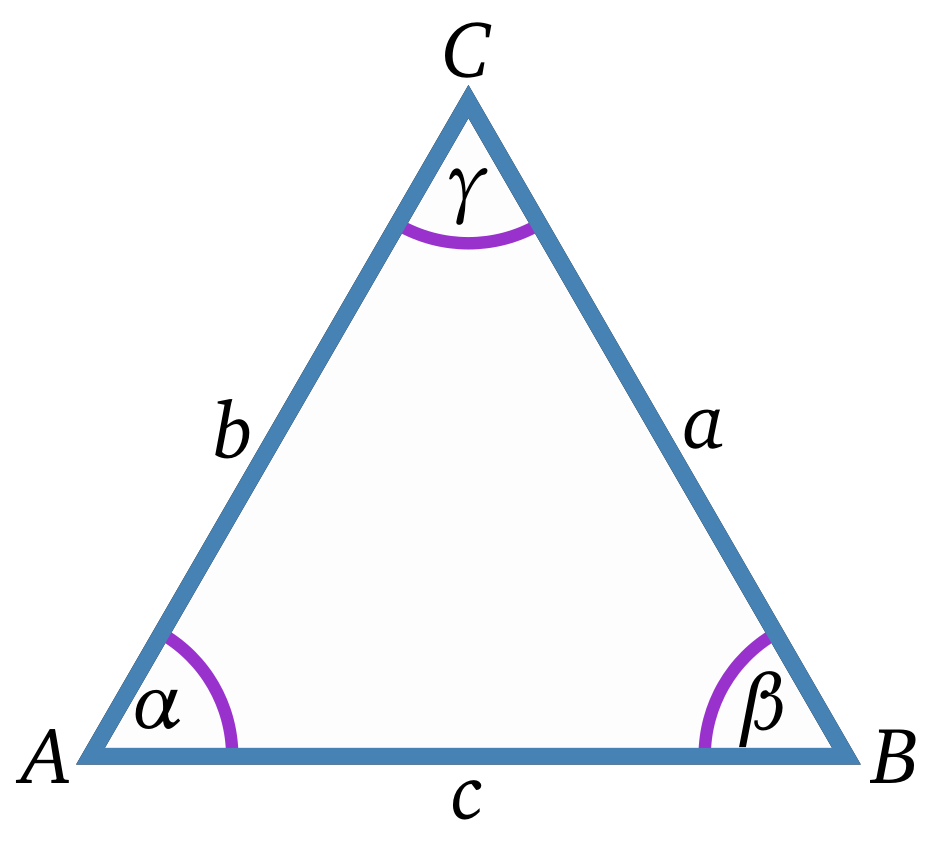
\includegraphics[width=0.75\textwidth,height=\textheight]{images/equilateral.png}
\caption{An equilateral triangle is one in which the three sides and
three angles are equal.}\label{fig:equilateral}
}
\end{figure}

The point at which a line meets another line is called a \emph{vertex},
which means a
\href{https://www.etymonline.com/search?q=vertex}{``turning point''}. By
convention, vertices (plural of vertex) are labelled with uppercase
letters like \(A\), \(B\), and \(C\). The lengths of the sides opposite
the vertices are assigned the lowercase labels \(a\), \(b\), and \(c\)
respectively. The angles have been labelled with the Greek letters
\(\alpha\), \(\beta\), and \(\gamma\). For all equilateral triangles,
\(a = b = c\), by definition, and by symmetry,
\(\alpha = \beta = \gamma\).

\hypertarget{degrees}{%
\subsection{Degrees}\label{degrees}}

On encountering geometry, we very likely proudly trotted out our set of
mathematical instruments, which would include a pair of compasses, a
protractor, one or two set squares, and a ruler or straight edge. Of
these, the protractor---that plastic semi-circle marked out in
\emph{degrees}---was the proud badge that proclaimed that we had left
behind arithmetic and progressed to geometry.

After we had learned to construct an equilateral triangle, using only
compasses and a straight edge---\emph{without measurement} by ruler---we
would take out the protractor to verify that each angle of an
equilateral triangle was indeed 60°. That small circle ° at the
top---the superscript---was called the \emph{degree sign}, and we could
then jubilantly celebrate our first rite of passage into geometry and
mathematical symbols.

\hypertarget{where-did-degrees-come-from}{%
\subsubsection{Where did degrees come
from?}\label{where-did-degrees-come-from}}

Surely, degrees did not come from a protractor, although we use one to
measure angles. How did degrees come about? With sixty degrees each in
an equilateral triangle, ninety in a right angle , 180° in a straight
line, and 360° in a full circle, how did degrees come to rule the roost
of angular measure in elementary school?

Why not 100° in a full circle, or half circle, or even a quarter circle,
also known as a right angle? Who imposed this measure upon us and what
is its basis?

My favourite explanation for 360° degrees equalling a full circle is
that the ancients estimated a solar year at around 360 days, and
assigned one degree for each day of the year. Even if inexact, the
number 360 had some
\href{https://en.wikipedia.org/wiki/Sexagesimal}{sexagesimal}\footnote{It
  appears that all measures of time, from seconds, minutes, and hours,
  to months and days in a year, are based on 60 or its factors or
  multiples.} charm as it could be divided by the first three primes 2,
3, 5, and by their products. Indeed, 360 = 2\textsuperscript{3} ×
3\textsuperscript{2} × 5. Accordingly, 360 has a large family of
factors: 1, 2, 3, 4, 5, 6, 8, 9, 10, 12, 15, 18, 20, 24, 30, 36, 40, 45,
60, 72, 90, 120, 180, and 360.

But beyond the approximation of a solar year, and the convenience of
ready division by its factors, the use of degrees as a unit of angular
measure is, to me, arbitrary. Who deemed the circle to be 360°, despite
it being very factor-friendly?

\hypertarget{from-triangles-to-circles}{%
\subsection{From triangles to circles}\label{from-triangles-to-circles}}

What is the root concept behind the idea of an angle? Harking back to
the etymology of the word vertex---and applying it to the equilateral
triangle---when one line \emph{changes direction} by sixty degrees, we
get the second line. These two lines form the angle. Therefore, a change
of direction may also be called \emph{turning} or \emph{rotation}.

The quintessential two-dimensional geometric figure that is associated
with rotation is of course the \emph{circle}. It is the most simple and
symmetrical two-dimensional figure we can construct. It is the path or
\emph{locus} traced out by a point that remains the \emph{same} distance
from a fixed point called the \emph{centre}. When a protractor is
centred on the centre of a circle, we can measure out degrees on the
circumference of the circle. So far so good. But what about that magic
number 360? Well, we are about to exorcise it now. \emojifont {😉}
\normalfont

\hypertarget{radians-as-an-alternative-to-degrees}{%
\subsection{Radians as an alternative to
degrees}\label{radians-as-an-alternative-to-degrees}}

One traumatic transition for the student of elementary mathematics is
when he or she is forced to abandon the warm comfort of degrees as
angular measure, and compulsorily made to embrace the cold and cruel
radian as \emph{the} angular measure forever afterward. Why this unfair
compulsion?

\hypertarget{using-circles-to-measure-angles}{%
\subsubsection{Using circles to measure
angles}\label{using-circles-to-measure-angles}}

Because the idea of an angle is related to rotation, it seems natural
that we should define angles using the circle as a basis, rather than
the triangles that we encountered at first.

It is a fact that the \emph{length} of a circle, or its
\emph{perimeter}, or its \emph{circumference}, \(C\), is always related
to its radius, \(r\), through the formula:
\begin{equation}\protect\hypertarget{eq:2pir}{}{
C = 2\pi r.
}\label{eq:2pir}\end{equation} And \(\pi\) is not \(\frac{22}{7}\) as we
were originally taught, but really a number whose precise expression
cannot be predicted or exhausted. The digits simply keep rolling on,
without pattern or end. But the beauty is that \(\pi\) is nevertheless a
unique number, a universal mathematical constant. It seems that Nature
has played a game on us by making the simple symmetrical circle have a
circumference that can only be approximated but never entirely known to
an unlimited precision.\footnote{\(\pi\), \(e\) the base of natural
  logarithms, \(\phi\) the golden ratio, along with a large pantheon of
  mathematical constants are irrational, and some are even possibly
  transcendental. Why Nature has this preference for the irrational is
  an intriguing question that needs an answer.}

\hypertarget{one-radian}{%
\subsubsection{One radian}\label{one-radian}}

So, how does one define a radian? If, on the basis of its name, you
guessed that it very likely involves the radius of a circle, your
suspicion is well-founded. \emph{One radian is the angle subtended at
the centre of a circle of radius one unit by an arc that is also one
unit long}. This is illustrated in \cref{fig:radian}.

\begin{figure}
\hypertarget{fig:radian}{%
\centering
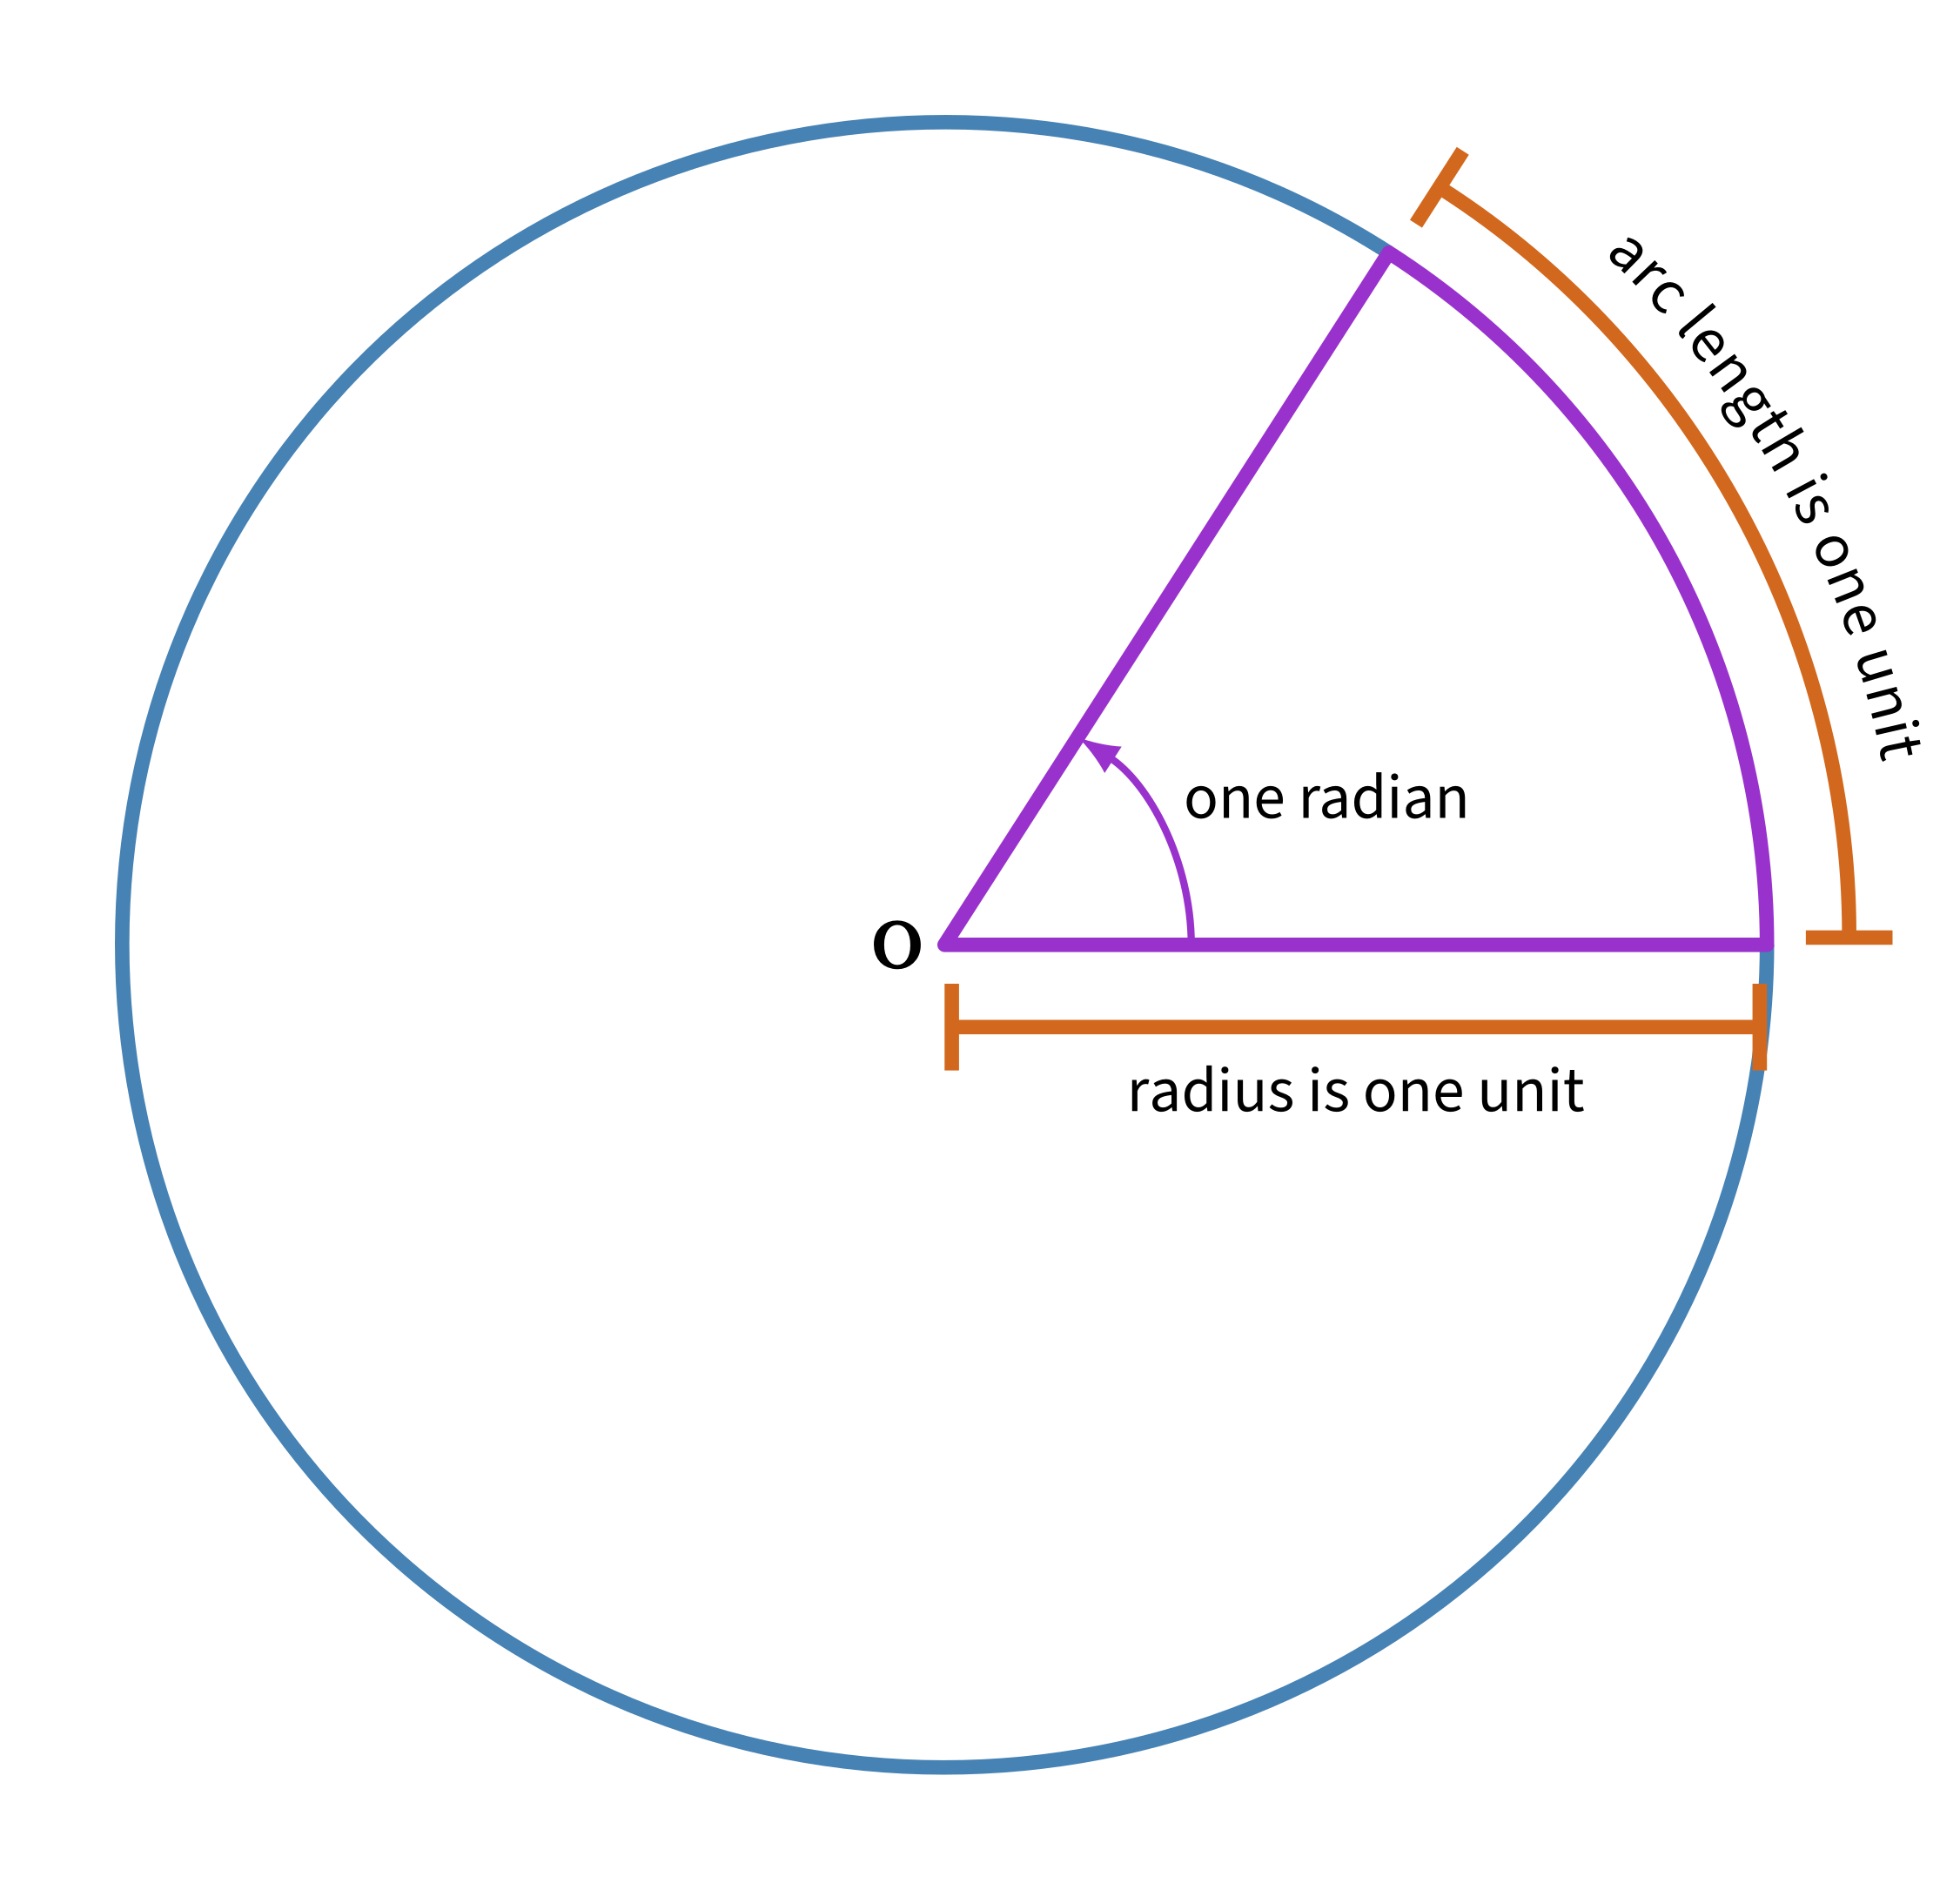
\includegraphics[width=0.8\textwidth,height=\textheight]{images/one-radian.png}
\caption{One radian is the angle subtended at the centre of a unit
circle by an arc of length equal to one unit.}\label{fig:radian}
}
\end{figure}

But what happens when our circle has a radius larger or smaller than one
unit? We will take up this case, after a short detour.

\hypertarget{congruence-and-similarity}{%
\subsubsection{Congruence and
similarity}\label{congruence-and-similarity}}

This is a mathematically non-rigorous digression on congruence and
similarity, both of which are first encountered in school in the context
of triangles, as shown in \cref{fig:similar}.

\begin{figure}
\hypertarget{fig:similar}{%
\centering
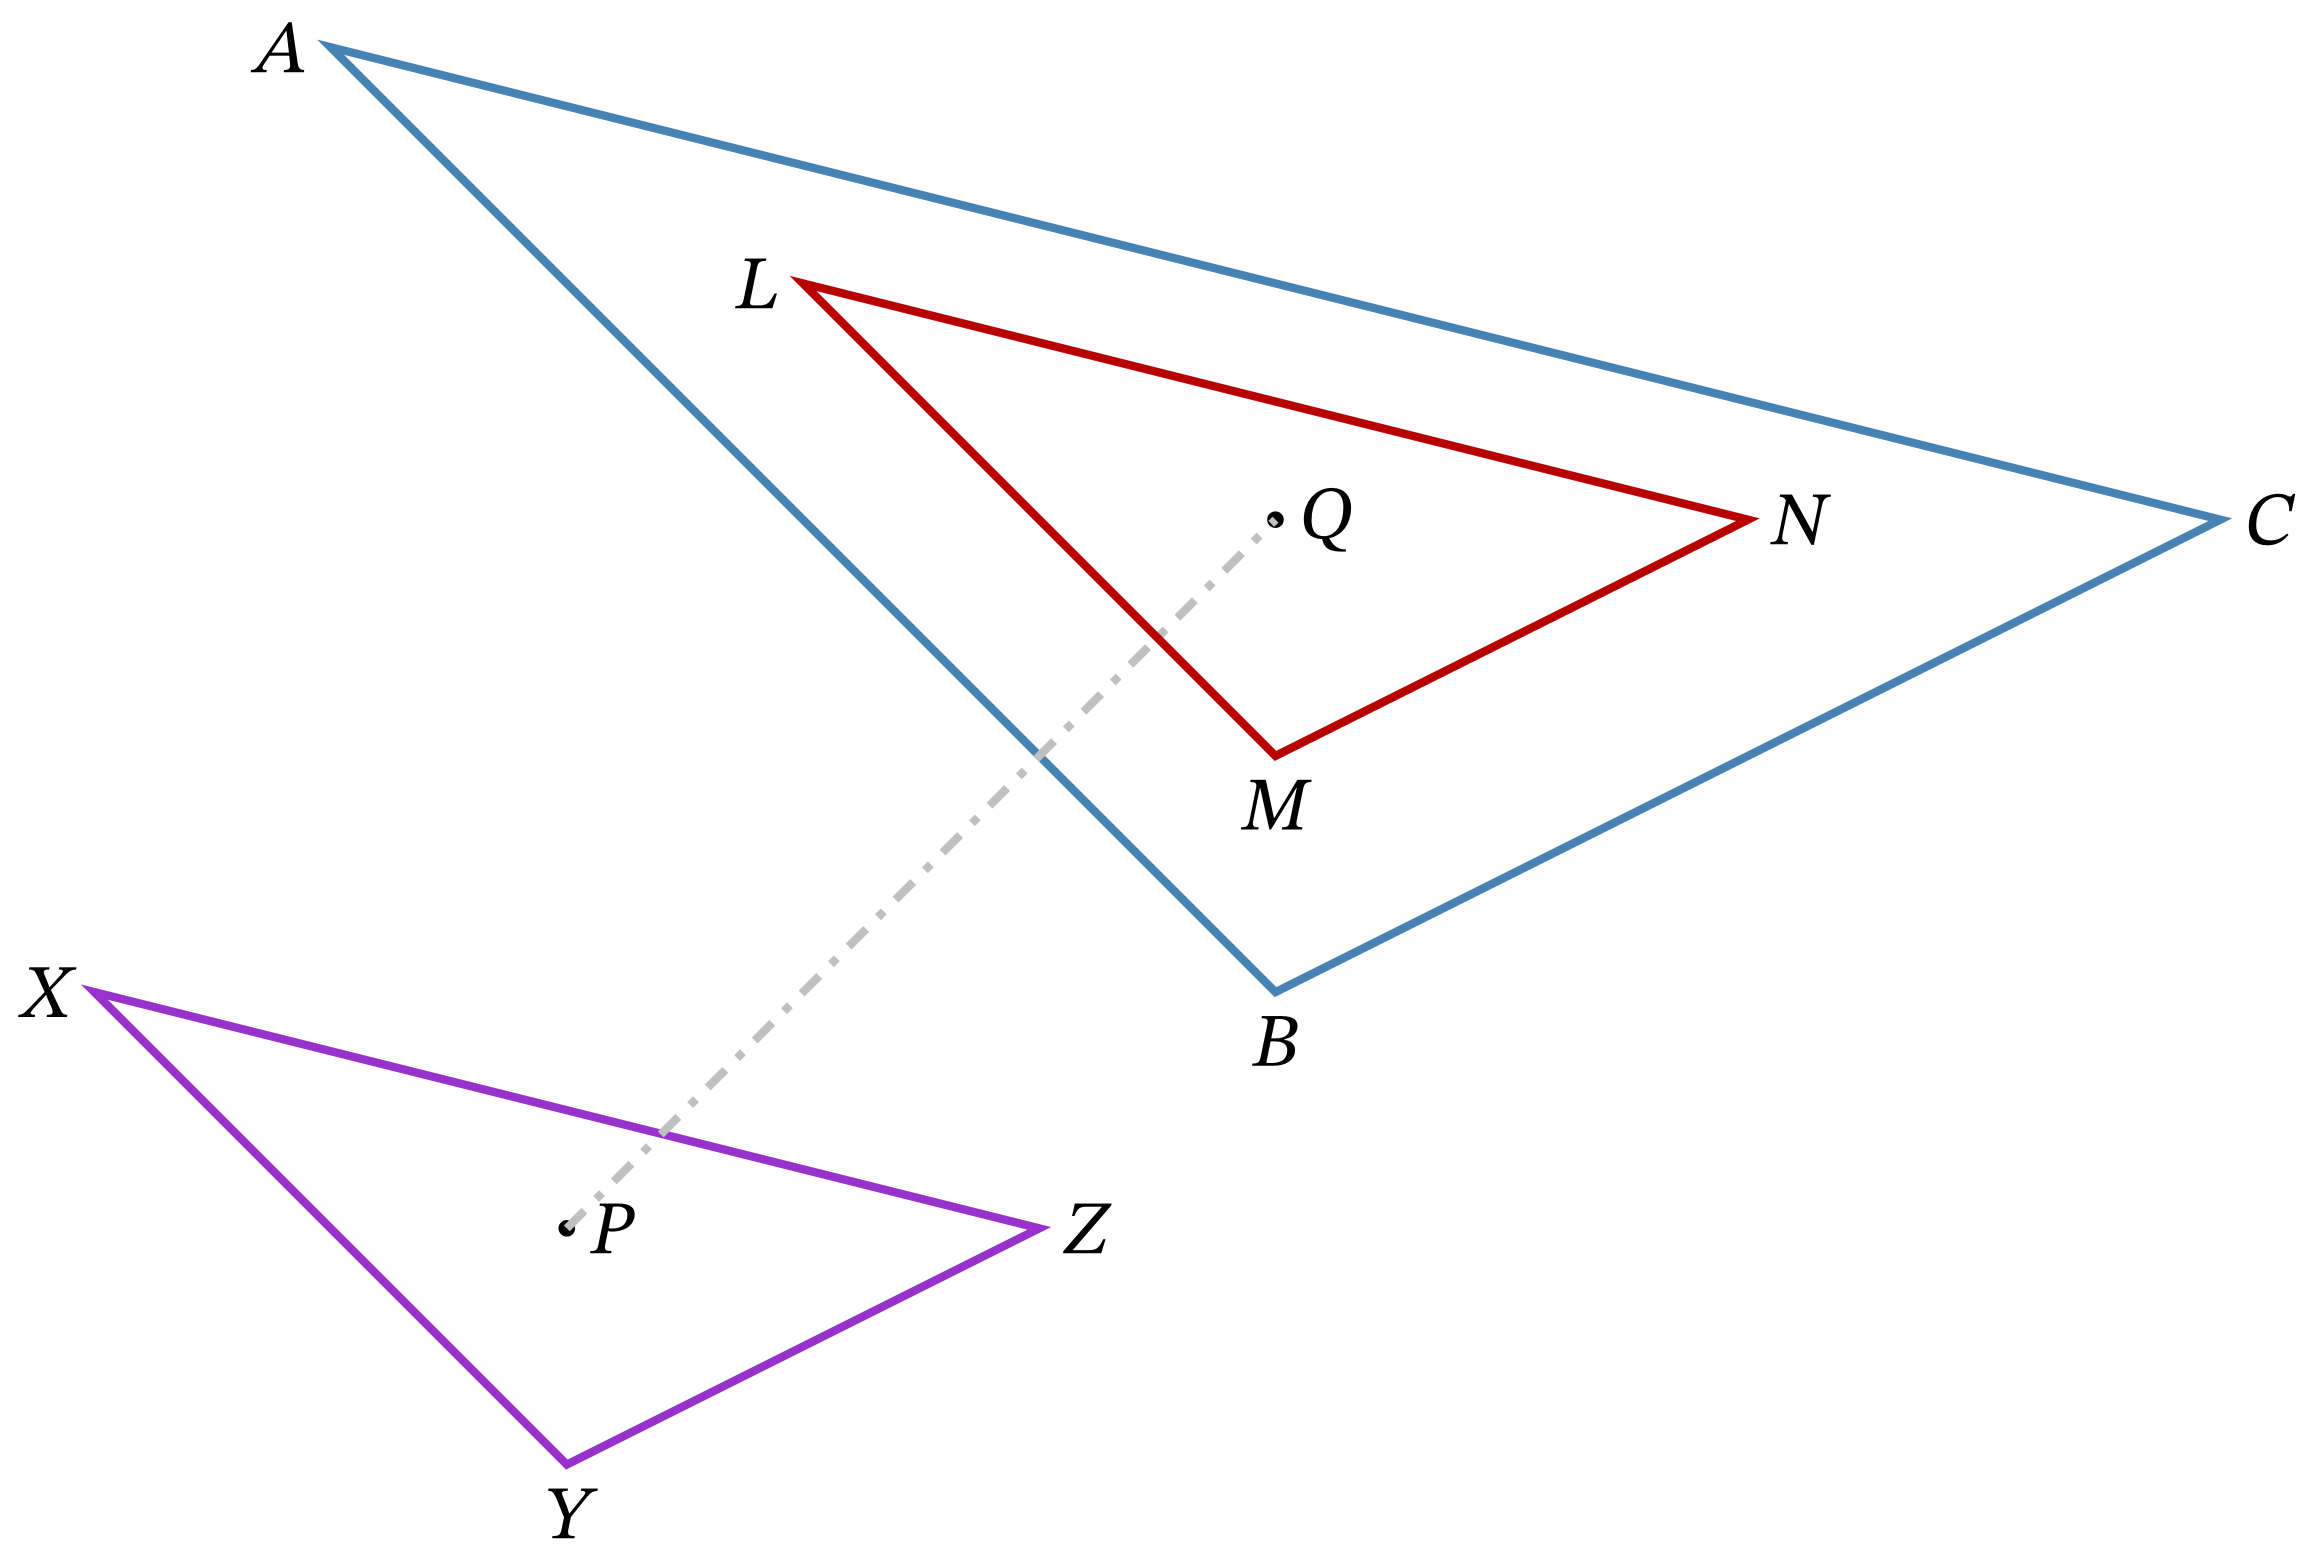
\includegraphics[width=0.7\textwidth,height=\textheight]{images/similar.png}
\caption{Similarity and congruence in the context of triangles. See the
text for the explanation.}\label{fig:similar}
}
\end{figure}

Consider the triangle \(XYZ\), and ignore for a moment triangle \(LMN\).
Suppose that \(XYZ\) is moved in the direction of the line \(PQ\) for a
distance equal to the length of \(PQ\). We would \emph{then} have the
triangle \(LMN\).

Triangle \(LMN\), being a shifted version of triangle \(XYZ\), is
identical with it, having identical respective angles and sides. Indeed,
if triangle \(XYZ\) were laid on top of \(LNM\), we
\href{https://www.merriam-webster.com/dictionary/tell\%20apart}{could
not tell them apart}. We say that triangle \(XYZ\) is \emph{congruent}
to triangle \(LMN\).

Any two-dimensional geometrical shape is congruent to another if the two
shapes may be superimposed\footnote{After any necessary translation and
  rotation.} on each other to visually demonstrate that they are
indistinguishable.

\emph{Similarity} is less restrictive than congruence and applies to
geometric objects that have the same shape but not necessarily the same
size. In \cref{fig:similar}, triangle \(ABC\) is similar to triangles
\(XYZ\) and \(LMN\).

Intuitively, if two objects are similar, one may \emph{zoom in} or
\emph{zoom out} on one object of the pair---without distortion---to
obtain a version that may be superimposed on the other object to
demonstrate that they are identical or congruent. In this case, we may
\emph{enlarge} triangle \(LMN\) until it attains the same size as
triangle \(ABC\). It will then be congruent to \(ABC\).

The ratios of the respective lengths of corresponding sides of similar
triangles are the same. In like fashion, the ratio of any arc length to
the radius of a circle is the same for all arcs subtending the
\emph{same} angle at the centre. For example, the ratio of the
circumference to the radius for two circles of radii \(r_1\) and \(r_2\)
will be \(\frac{2\pi r_1}{r_1} =\frac{2\pi r_2}{r_2} = 2\pi\), which is
a constant.\footnote{This also demonstrates that a full circle
  corresponds to an angle of 360° or \(2\pi\) radians.} This is a
consequence of the fact that \emph{all circles are similar to each
other}.

What other classes of geometrical objects can you think of that are
similar to each other within their class?\footnote{All circles are
  similar, as are all equilateral triangles, all squares, and indeed,
  all regular \(n\)-gons, and all parabolas.}

\hypertarget{radians-as-angular-measure}{%
\subsection{Radians as angular
measure}\label{radians-as-angular-measure}}

Consider \cref{fig:general} in which two circles having different radii
are shown.

\begin{figure}
\hypertarget{fig:general}{%
\centering
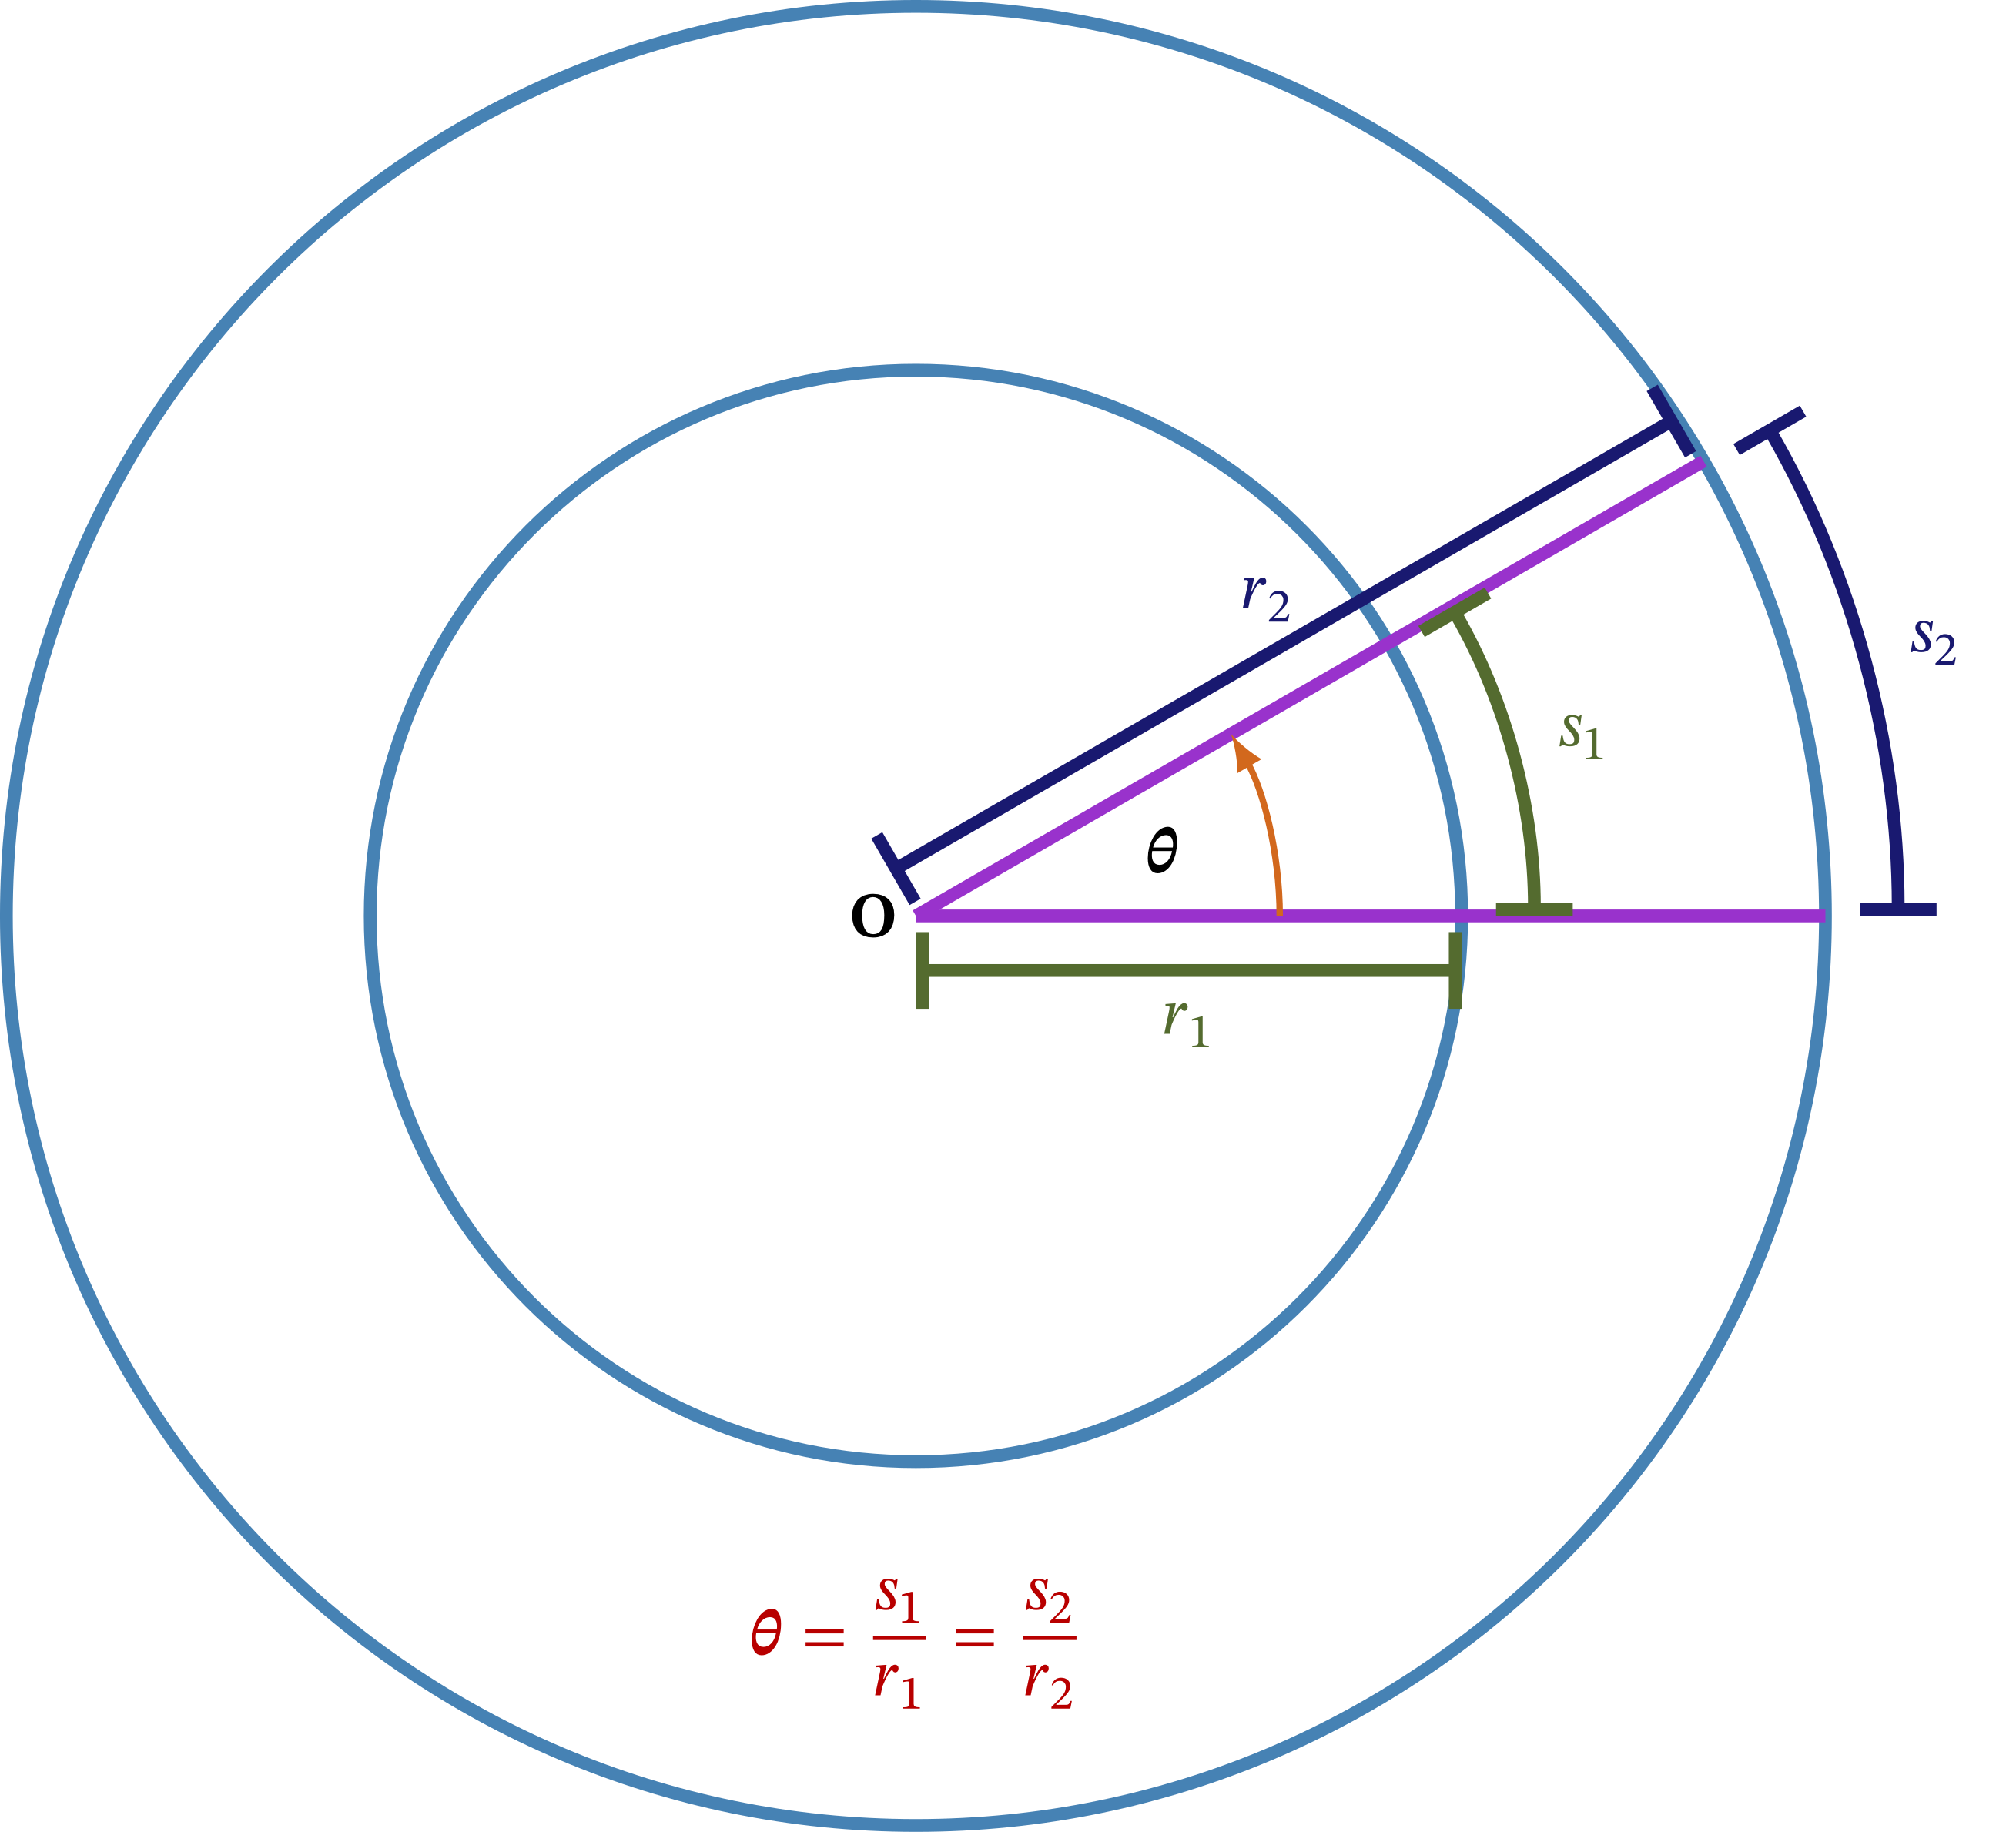
\includegraphics[width=0.65\textwidth,height=\textheight]{images/general-radian.png}
\caption{Generalized measure of an angle in radians. The arbitrary angle
\(\theta\) in radians is defined as
\(\theta = \frac{s_1}{r_1} = \frac{s_2}{r_2}\). The equality is valid
because all circles are similar to each other.}\label{fig:general}
}
\end{figure}

We are now ready to define the value of any angle in radians. Consider a
circle of radius \(r\). Let an arc of arbitrary length \(s\) subtend an
angle of \(\theta\) at the centre. The angle \(\theta\) in radians is
\emph{defined} to be: \begin{equation}\protect\hypertarget{eq:defrad}{}{
\theta \triangleq \frac{\text{arc length}}{\text{radius}} = \frac{s}{r}.
}\label{eq:defrad}\end{equation}

By dividing the arc length by the radius, we have in effect
\emph{normalized} radian measure, and removed any trace of
arbitrariness\footnote{Such as dependence on the radius of the circle.}
in its definition. And that is why we started out with
\cref{fig:radian}, which dealt with a circle of radius one unit. We know
from \cref{fig:general} that similarity guarantees that the value
\(\frac{s}{r}\) for any given \(\theta\) is constant for all circles
regardless of radius.

Note that the value of \(\theta\) is a ratio of two lengths and is
therefore dimensionless in the sense of Physics. Although it may be
considered a unitless \emph{pure number}
\href{https://en.wikipedia.org/wiki/Radian}{the SI units do define the
\emph{radian} as the \emph{SI unit of angular measure}}.

In summary, we have the following:

\begin{enumerate}
\tightlist
\item
  Radian angular measure is directly proportional to arc length on the
  circle.
\item
  This measure is independent of the radius of the circle.
\item
  The resulting ``unit'' is really a unitless ratio of two lengths.
\item
  Since 360° equals \(2\pi\) radians, 1° approximately equals
  0.017453292 radians. Likewise, 1 radian equals approximately
  57.29577951°.\footnote{These conversion factors must dispel any
    mystique attached to radians vis-a-vis degrees.}
\end{enumerate}

By defining radians as above, we remove the arbitrariness associated
with 360° for a full circle. But the mathematical elegance and rigour
conferred by radians comes at a cost. The angle of a full circle is
\(2\pi\), which is a computationally inconvenient number to say the
least.

If you think about it, the size of an angle in radians is expressed as a
\emph{ratio of two lengths}. But we have encountered angles being
associated with ratios of lengths elsewhere in mathematics as well. Such
ratios are familiar to us from \emph{trigonometry} where the \(\sin\),
\(\cos\), and \(\tan\) functions are expressed as the ratios of lengths
in a right-angled triangle. We review this relationship next.

\hypertarget{trigonometric-functions}{%
\subsection{Trigonometric functions}\label{trigonometric-functions}}

Trigonometric functions are one of the workhorses of applied
mathematics. They arose from the study of right-angled triangles. The
three standard trigonometric functions are called \emph{sine},
\emph{cosine}, and \emph{tangent}. They are represented by the
abbreviated functional names \(\sin\), \(\cos\), and \(\tan\) when used
in mathematics. \cref{fig:trig} shows the pictorial definitions of these
three trigonometric functions. Notice particularly how these function
values are the unitless \emph{ratios of two lengths}, just as with
radians.

\begin{figure}
\hypertarget{fig:trig}{%
\centering
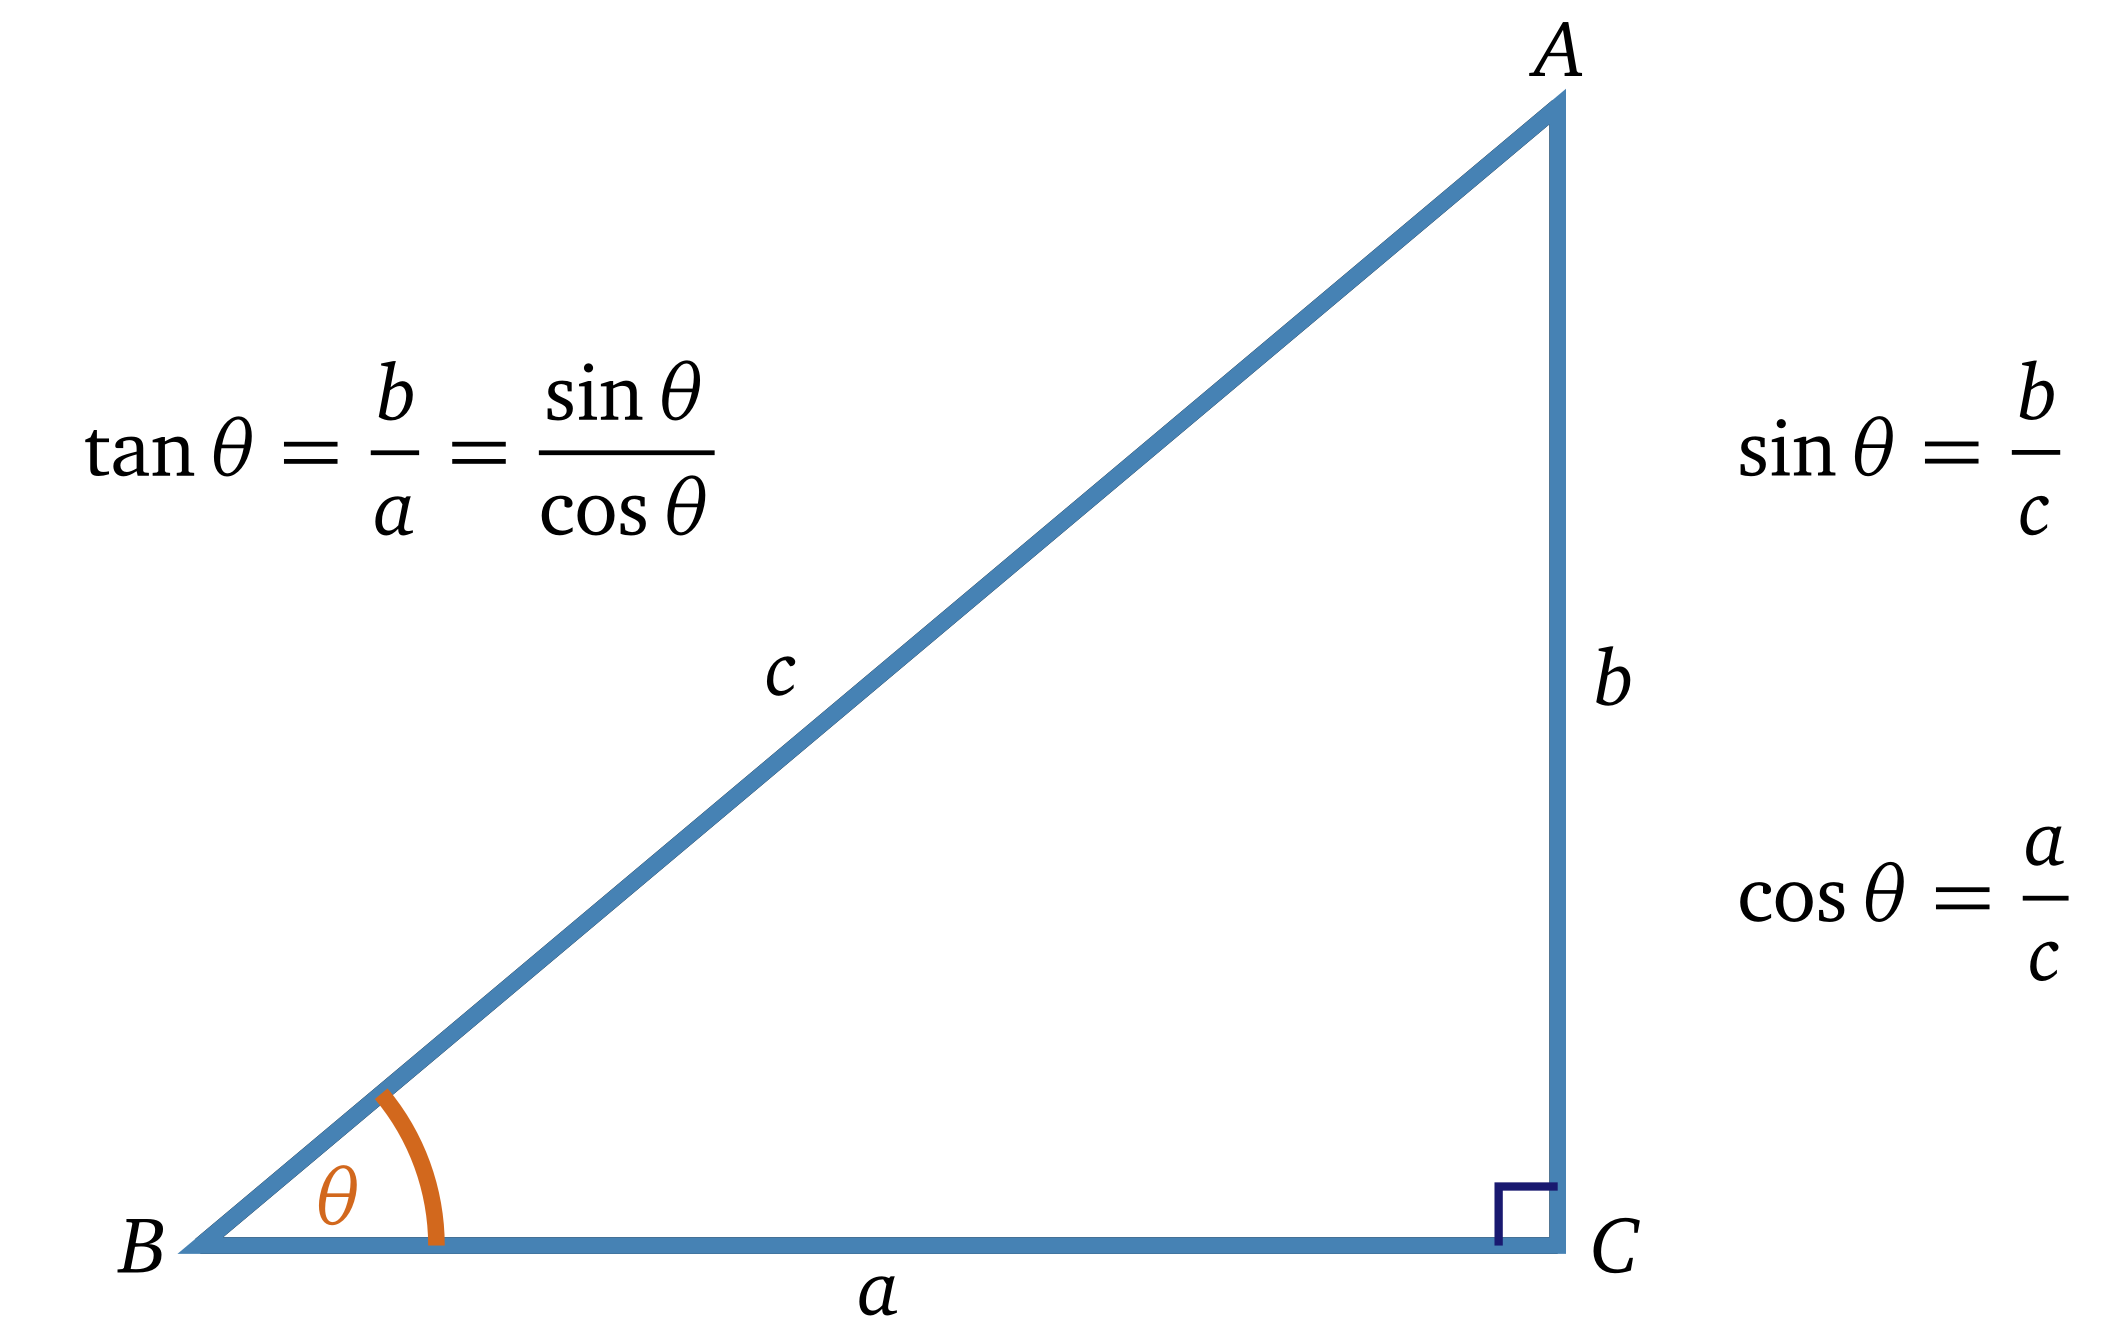
\includegraphics[width=0.9\textwidth,height=\textheight]{images/trig.png}
\caption{Trigonometric functions defined as ratios of lengths of sides
in a right-angled triangle.}\label{fig:trig}
}
\end{figure}

\hypertarget{the-circular-functions}{%
\subsection{The Circular Functions}\label{the-circular-functions}}

The trigonometric functions are also called the \emph{circular}
trigonometric functions, uniting the circle \emph{and} the triangle as
their progenitors. We will briefly review that relationship here, to
better understand not only the terminology but also the hidden
relationships between the triangle and the circle.\footnote{The
  equilateral triangle is the regular \(n\)-gon with the smallest number
  of sides and the circle is the limiting case of an \(n\)-gon when
  \(n\) tends to infinity. The trigonometric functions are the children
  of these unlikely parents, at the extreme ends of the \(n\)-gon
  spectrum.}

I used to wonder why the word \emph{tangent} was used for the name of a
trigonometric function because a circle was not involved in its
definition; a triangle was. But when the three standard trigonometric
functions are viewed vis-a-vis a unit circle, the mystery behind the
nomenclature is revealed.

The radian was introduced here using a \emph{unit circle}. The same
helpful unit circle will serve to relate the triangle and the circle to
the trigonometric functions, as illustrated in \cref{fig:unit} below.

\begin{figure}
\hypertarget{fig:unit}{%
\centering
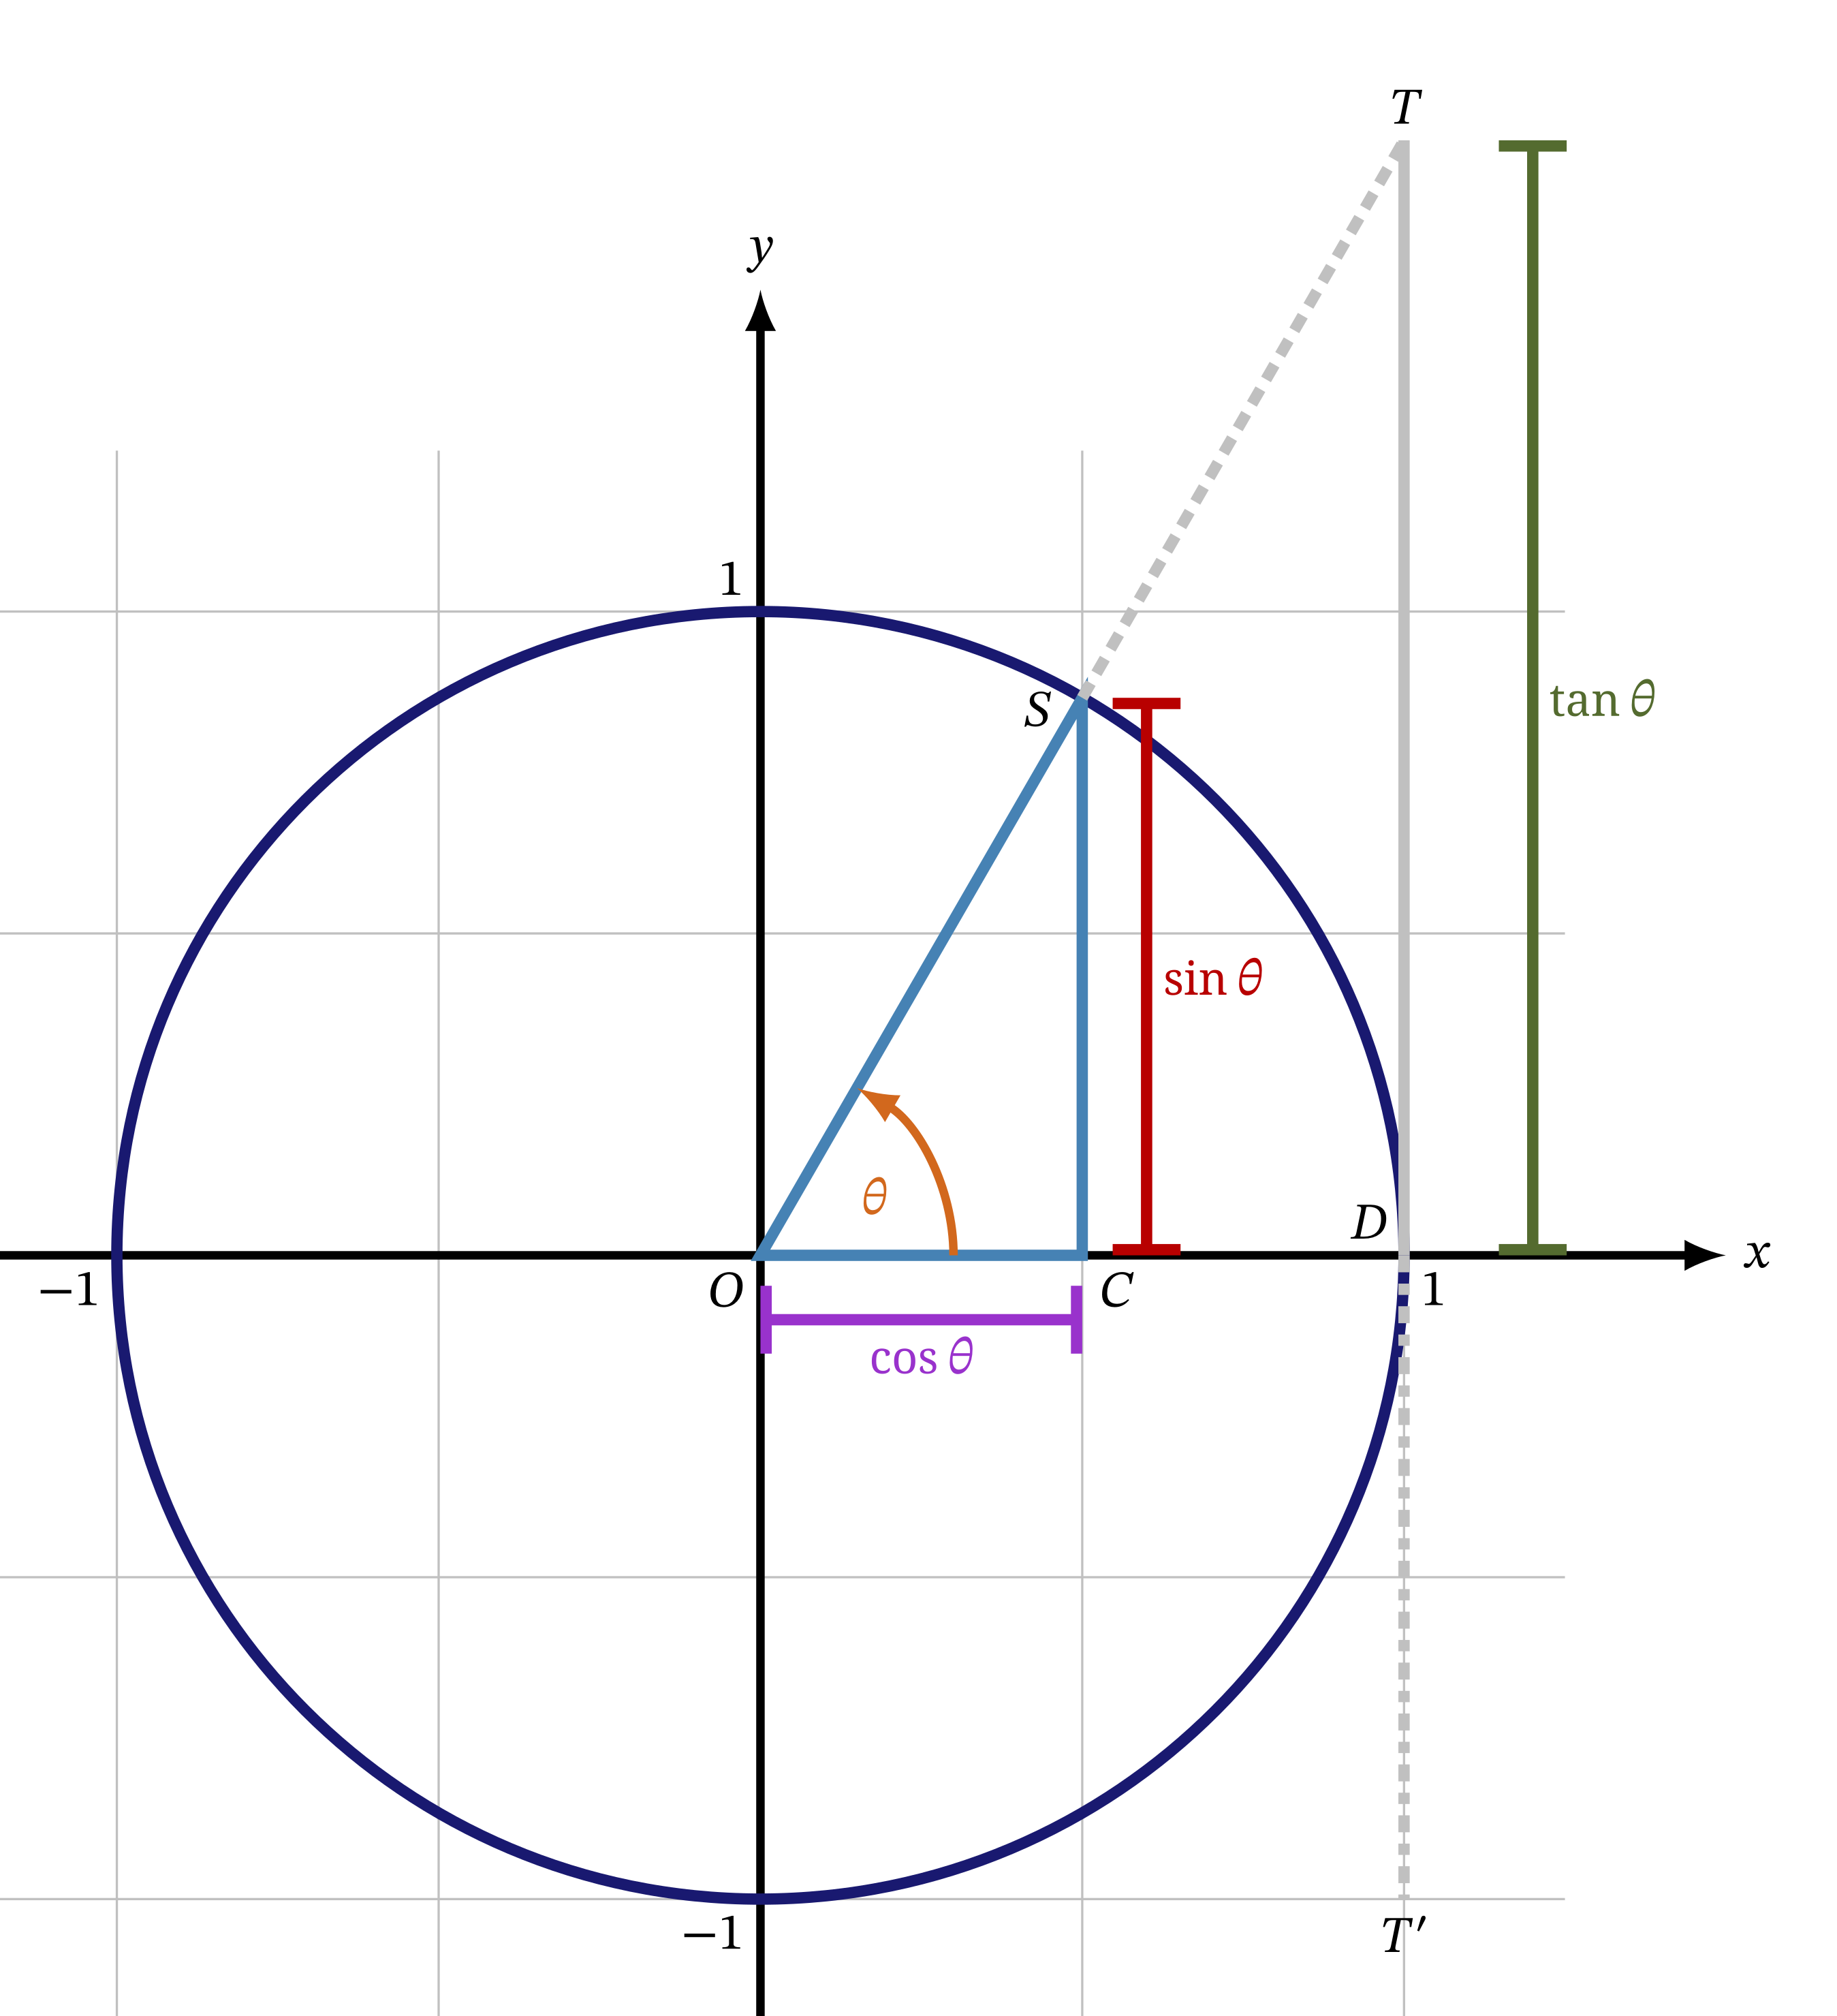
\includegraphics[width=0.85\textwidth,height=\textheight]{images/unit-circle.png}
\caption{A pictorial representation of the unit circle, the three
standard trigonometric functions, and their inter-relationships. See the
text for a full explanation.}\label{fig:unit}
}
\end{figure}

\cref{fig:unit} shows a unit circle drawn on the two-dimensional
coordinate plane with \(x\) and \(y\) axes and grid markings. The centre
of the circle is \(O\) and \(S\) is a variable point on the
circumference of the circle, that makes a counter-clockwise angle
\(\theta\) with the positive \(x\)-axis. As \(\theta\) varies, so does
the position of \(S\) on the circle.

The line \(OS\) is a radius and therefore one unit in length. The
perpendicular from \(S\) to the \(x\)-axis meets it at \(C\). Referring
to \cref{fig:trig}, we may say \(\cos\theta = \frac{OC}{OS} = OC\) since
\(OS = 1\). Accordingly, the \(x\)-coordinate of \(S\) is
\(\cos\theta\). Likewise, \(\sin\theta = \frac{SC}{OS} = SC\). Thus, the
\(y\)-coordinate of \(S\) is \(\sin\theta\).

\emph{\(S\) is therefore the point with coordinates
\((\cos\theta, \sin\theta)\)}.

Note that since the coordinates of \(S\) are confined to the unit
circle, the values of \(\sin\theta\) and \(\cos\theta\) are confined to
the closed interval \([-1, 1]\), i.e.~they perforce have values lying
between \(-1\) and \(1\), both inclusive. From \cref{fig:unit}, we see
that \((\cos\theta, \sin\theta)\)---which represent the coordinates of
\(S\)---take on signed values in accordance with the signs of \(x\) and
\(y\) in the respective quadrants. One could also view the associated
\emph{lengths} as signed values.

\hypertarget{the-tangent}{%
\subsubsection{The tangent}\label{the-tangent}}

The really insightful revelation from \cref{fig:unit} comes from looking
at \(\tan\theta\). Have you ever wondered why the ratio
\(\tan\theta = \frac{\sin\theta}{\cos\theta}\) is called the
\emph{tangent}?

Recall from geometry that a straight line and a circle might lie
relative to each other in three different ways as shown in
\cref{fig:chord-tangent}.

\begin{figure}
\hypertarget{fig:chord-tangent}{%
\centering
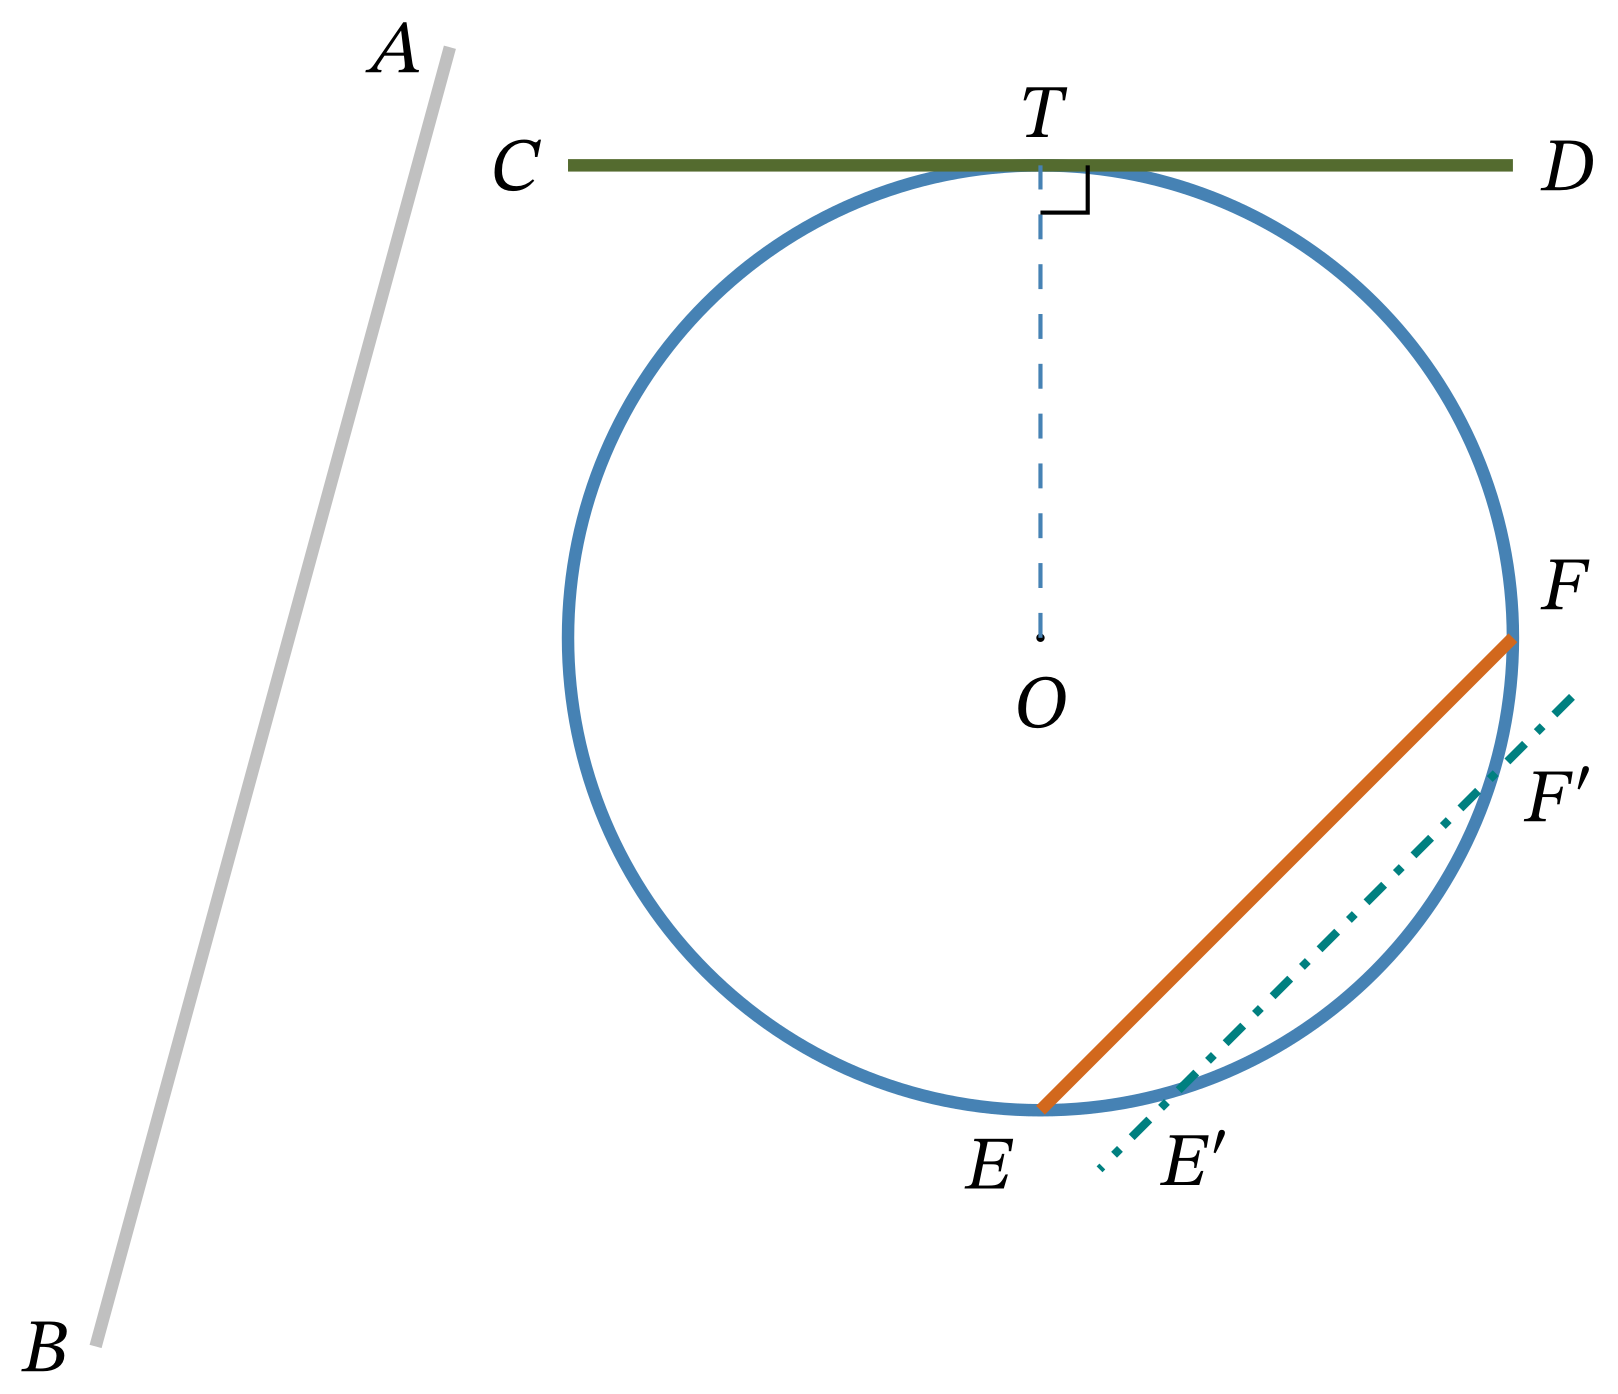
\includegraphics[width=0.7\textwidth,height=\textheight]{images/chord-tangent.png}
\caption{The three different ways in which a circle and line may lie
relative to each other. See the text for the
explanation.}\label{fig:chord-tangent}
}
\end{figure}

The line \(AB\) does not cut or \emph{intersect} the circle at all. The
line \(EF\) cuts the circle at \emph{two} points, \(E\) and \(F\), and
is called a
\href{https://en.wikipedia.org/wiki/Chord_(geometry)}{chord}. When the
line \(EF\) moves parallel to itself toward the circumference of the
circle, we get the chord \(E'F'\). Eventually the points \(E'\) and
\(F'\) will coincide and the line will cut the circle at one and only
one point.

This case is illustrated by the line \(CTD\) which cuts the circle at
only one point, \(T\). \(CTD\) is called a
\href{https://en.wikipedia.org/wiki/Tangent_lines_to_circles}{tangent
(line)} to a circle and \(T\) is the point of tangency.\footnote{Therefore,
  the tangent is a limiting case of a chord.} Note that the radius
\(OT\) is perpendicular to the tangent \(CDT\).

With that out of the way, we know from \cref{fig:trig}, that the tangent
is the ratio of the lengths of the opposite side to the adjacent side,
which in \cref{fig:unit} translates to \(\tan\theta = \frac{SC}{OC}\).
But the denominator in this case, \(OC\), is not \(1\) like it was for
the other two trigonometric ratios. To work around this, with reference
to \cref{fig:unit}, we construct the triangle \(ODT\) thus:

\begin{enumerate}
\def\labelenumi{\alph{enumi}.}
\tightlist
\item
  Extend\footnote{Extending a line used to be called \emph{producing a
    line} but that usage has now slipped into relative obscurity.} the
  line \(OC\) to intersect the circle at the point \(D\) which is
  \((1, 0)\). \(OD\), being a radius, has unit length.
\item
  Draw a tangent \(T'DT\) to the circle at \(D\).
\item
  Extend the radius \(OS\) to intersect the tangent at the point \(T\).
\end{enumerate}

Because the triangle \(ODT\) is similar to triangle \(OCS\), we can
assert that the ratios of corresponding sides are equal. Thus,
\begin{equation}\protect\hypertarget{eq:tangent}{}{
\tan\theta = \frac{CS}{OC} = \frac{DT}{OD} = DT
}\label{eq:tangent}\end{equation} bearing in mind that, like \(OS\),
\(OD\) is also a radius of unit length. We resorted to this construction
for the following reasons:

\begin{enumerate}
\tightlist
\item
  Because \(T'DT\) is tangent to the circle, the angle \(ODT\) is a
  right angle.
\item
  The triangles \(OCS\) and \(ODT\) are therefore similar.
\item
  The length of \(OC\) is not one unit, but that of \(OD\) is one unit.
\end{enumerate}

From \cref{fig:unit} the length of the \emph{tangent line} \(DT\) is
equal to \(\tan\theta\), explaining the nomenclature.

Therefore, the value of the tangent function for an angle \(\theta\) may
be determined geometrically by extrapolating the radius \(OS\) until it
intersects the tangent to the circle at \(D\) at a point called
\(T\).\footnote{One could also extraolate in the \emph{opposite}
  direction to intersect at, say, the point T'.} The length \(DT\) is
the value of \(\tan\theta\).

Note, though, that \(\tan\theta\) is a length \emph{outside the unit
circle} and is therefore not constrained to take on values between
\(-1\) and \(1\). Indeed, as \(\theta\) starts increasing in the first
quadrant of the unit circle, you will notice that as \(OS\) approaches
the \(y\)-axis and as \(\theta\) approaches \(\frac{\pi}{2}\) (or 90°,
if you are still attached to degrees), the line \(OS\) is increasingly
aligned with \(DT\). At \(\theta=\frac{\pi}{2}\), \(OS\) is parallel to
\(DT\) and
\href{https://en.wikipedia.org/wiki/The_Ballad_of_East_and_West}{``never
the twain shall meet''}. Loosely speaking, parallel lines are only
supposed to ``meet at infinity'' and that is why \(\tan\frac{\pi}{2}\)
is said to be ``infinite'' at that point. I find this geometric
explanation---of why \(\tan\theta\) does not assume a finite value at
\(\theta=\frac{\pi}{2}\)---most fulfilling.

When \(\theta\) is in the third quadrant, for instance, \(OS\)
extrapolated in the negative \(y\) direction will not intersect the
tangent \(DT'\) in the negative \(y\) direction as they diverge. So, the
line \(SO\) must be produced in the positive \(y\) direction to once
more intersect the tangent \(T'DT\) at \(T\). That explains why tangents
of angles in the third quadrant are positive.

\hypertarget{the-trigonometric-functions}{%
\subsection{The trigonometric
functions}\label{the-trigonometric-functions}}

By moving from triangles to the unit circle on coordinate axes, we have
enabled \(\theta\) to take on any value between 0 and \(2\pi\) radians.
The \emph{trigonometric ratios} have been unshackled from the triangle
to become the \emph{trigonometric functions} which can take on
\emph{any} real number as arguments. The graphs of the three standard
trigonometric functions are shown in \cref{fig:threegraph}.

\begin{figure}
\hypertarget{fig:threegraph}{%
\centering
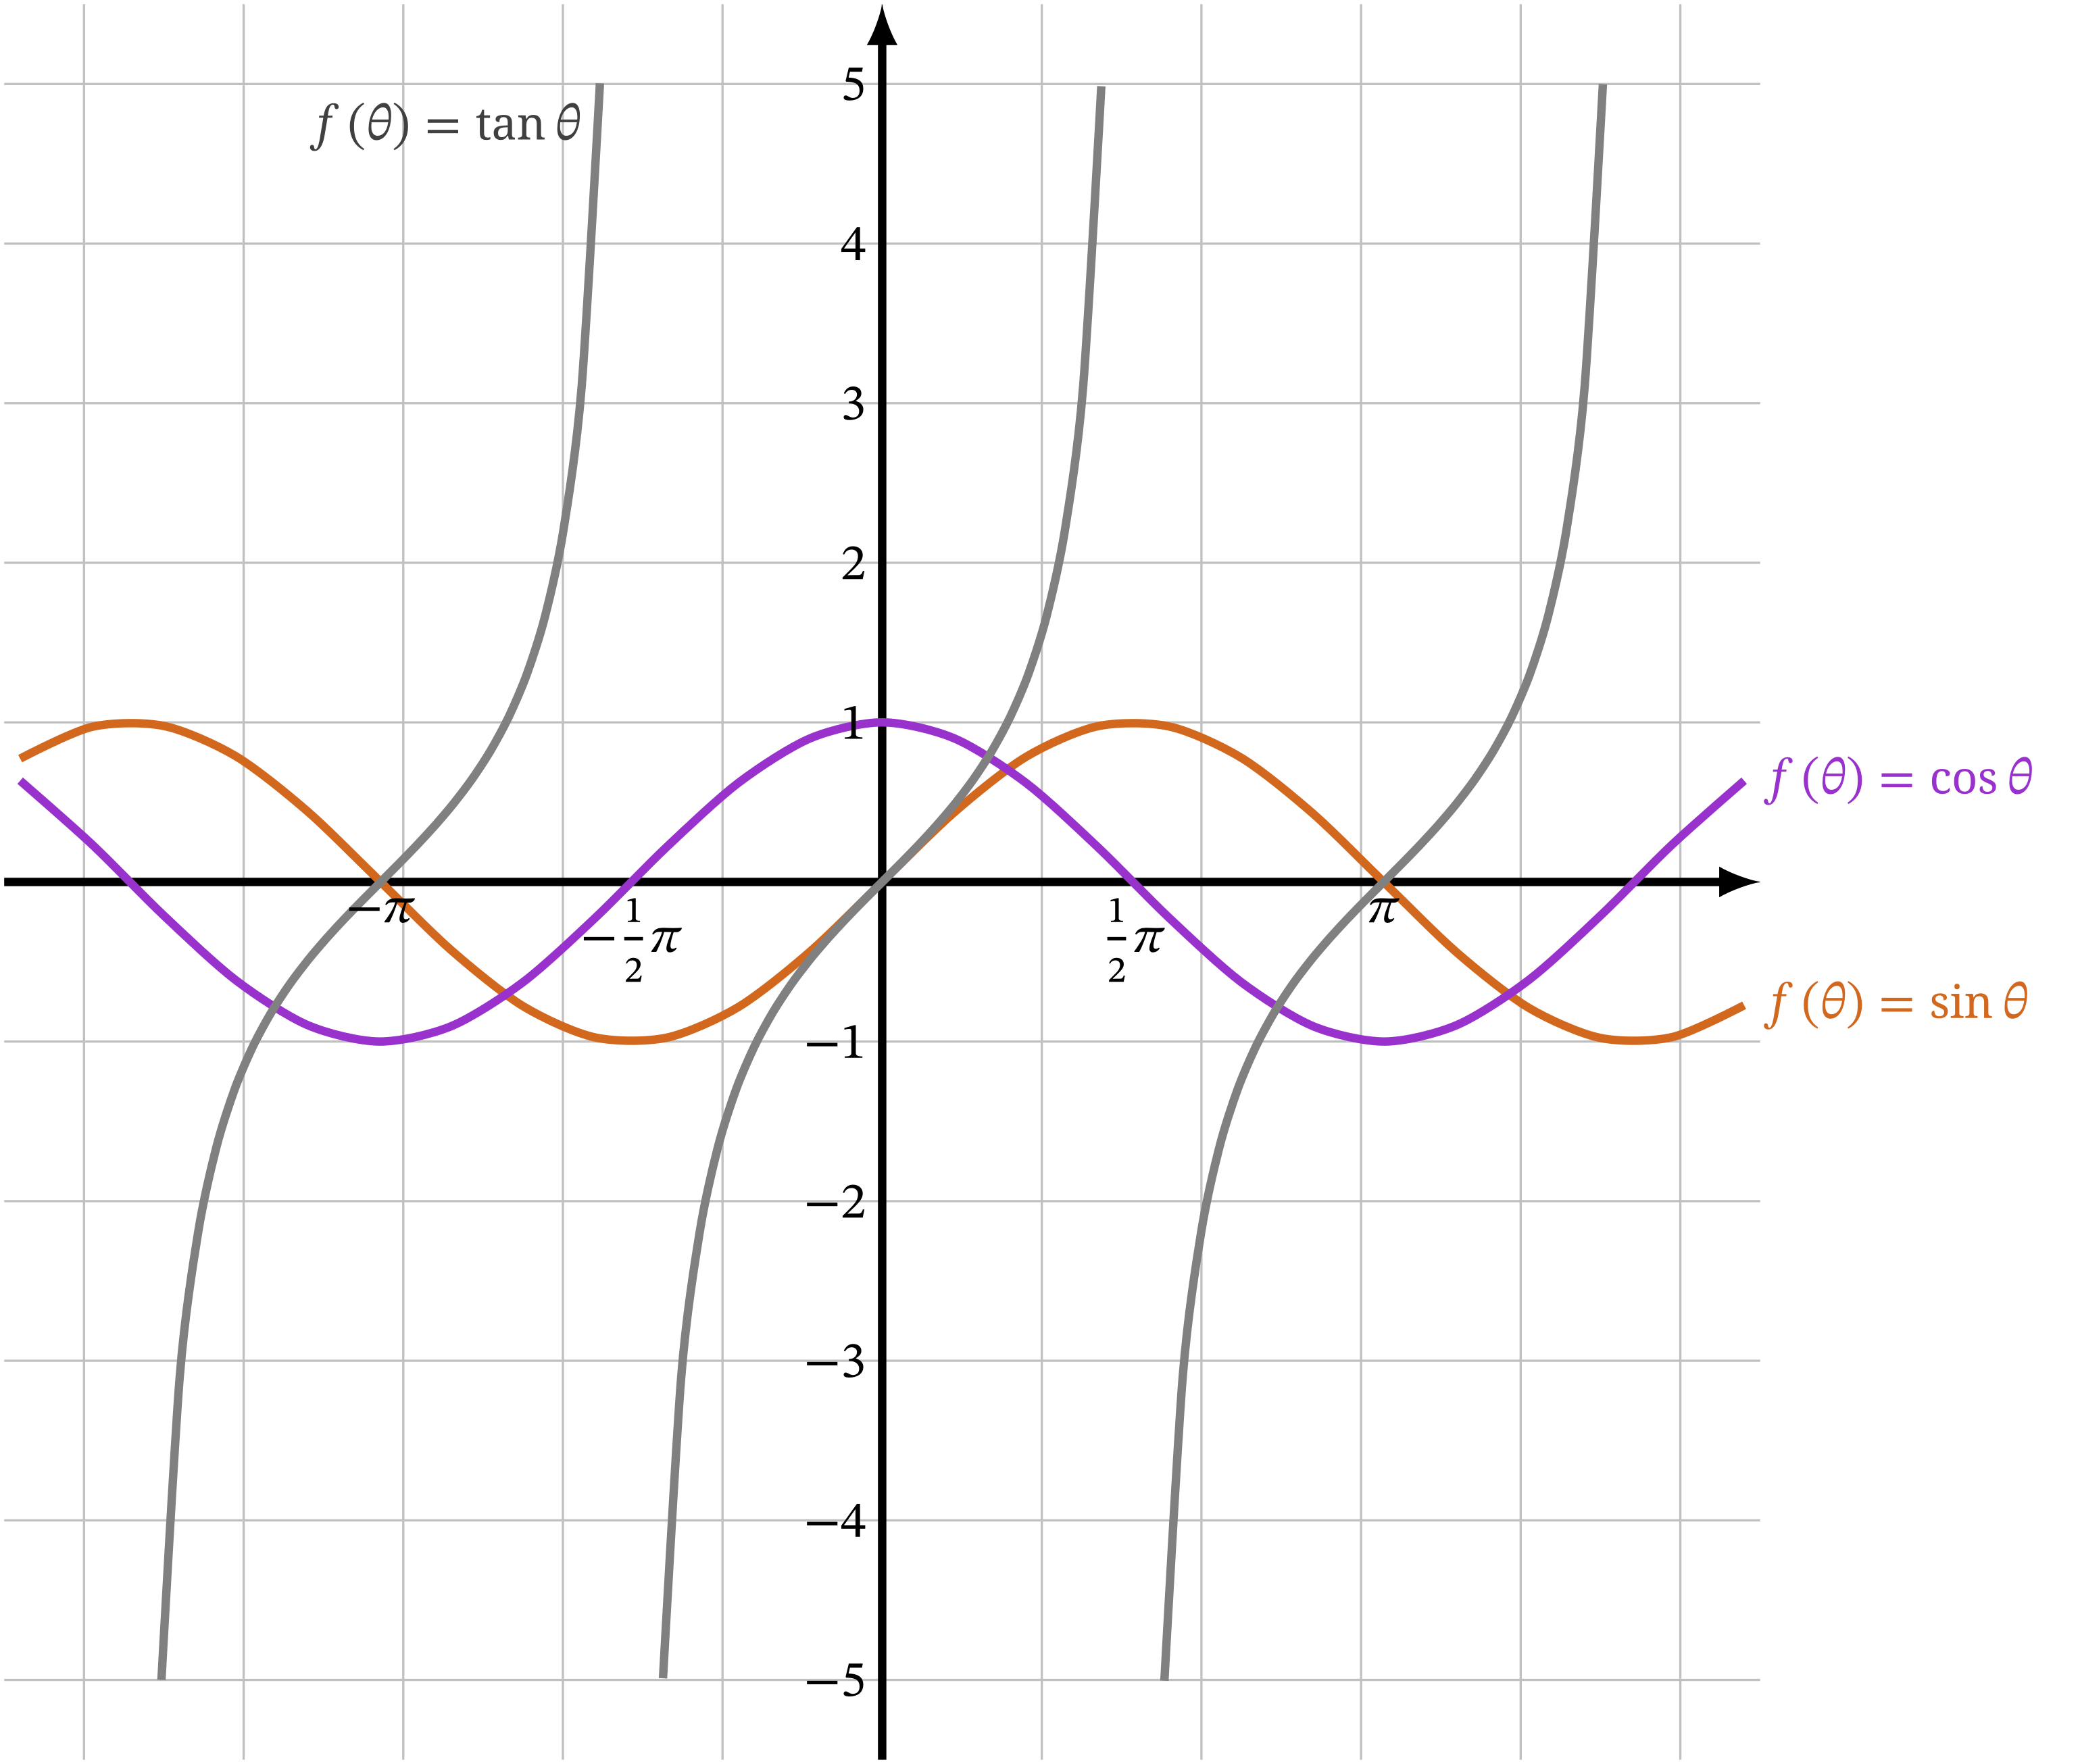
\includegraphics[width=0.9\textwidth,height=\textheight]{images/threegraph.png}
\caption{Graphs of the three trigonometric functions. Notice how
\(\sin\) and \(\cos\) are bounded in their values, but \(\tan\) is not.
There are discontinuities for
\(\theta=\frac{2n+1}{2}\pi\).}\label{fig:threegraph}
}
\end{figure}

Note that when \(\theta = 2\pi\) radians, we cannot really distinguish
it from \(\theta=0\) radians. The trigonometric functions therefore
repeat themselves every time the point \(S\) in \cref{fig:unit}
completes a full circle: they are
\href{https://mathworld.wolfram.com/PeriodicFunction.html}{\emph{periodic}}
with a period of \(2\pi\). So, one angle may
\href{https://www.thefreedictionary.com/masquerade}{masquerade} as
another unless we have accounting devices to optionally add \(2n\pi\) to
it with the
\href{https://dictionary.cambridge.org/dictionary/english/proviso}{proviso}
that \(n\) is an integer. And this concept is a
\href{https://www.dictionary.com/browse/segue}{segue} to power series
expansions of trigonometric functions, their use in calculus, and later
on, in Fourier series.

\hypertarget{power-series-for-trigonometric-functions}{%
\subsection{Power series for trigonometric
functions}\label{power-series-for-trigonometric-functions}}

This is where the plot really thickens.

Both the statements \(\sin(30°)=0.5\) and \(\sin(\frac{\pi}{6})=0.5\)
are factually correct and perfectly acceptable. We will not be
committing any mathematical heresies through either
statement.\footnote{Note that while it is mandatory to affix the degree
  sign as a superscript, radians being pure numbers do not require any
  special identification.}

But it is possible to express trigonometric functions in terms of power
series in which an argument in degrees would be inadmissible. It is only
after we cross this threshold in mathematics that radians truly come
into their own, after which there is ``no going back to the old ways''.

I will now do a bit of hand-waving and say that it has been
proved\footnote{Search the web for Taylor Series or Maclaurin series,
  thinking of it as a treasure hunt and enrich yourself with that
  knowledge!} that:

\begin{equation}\protect\hypertarget{eq:sineseries}{}{
\sin\theta = \theta - \frac{\theta^3}{3!} + \frac{\theta^5}{5!} - \frac{\theta^7}{7!} + \cdots
}\label{eq:sineseries}\end{equation}

where the dots at the end of \cref{eq:sineseries} tell us to imagine
that this series \emph{never ends but goes on forever} following the
pattern shown. \cref{eq:sineseries} demonstrates a paradox: a
trigonometric function is not a polynomial; yet a trigonometric function
may be expressed as an infinite polynomial. Infinity has this beguiling
attribute of ``enabling the impossible.''

Recall that if a number is less than one, raising it to a power greater
than one makes it smaller than it originally was. So, when \(\theta\) is
very close to zero, the higher powers on the right hand side (RHS) of
\cref{eq:sineseries} become smaller and smaller, and may be ignored
without much loss in accuracy. In this case, we may assert that:

\begin{equation}\protect\hypertarget{eq:sinesmalltheta}{}{
\sin\theta\approx\theta \:\text{for}\: \lvert\theta\rvert \to 0.
}\label{eq:sinesmalltheta}\end{equation}

In English this expression means that for vanishingly small values of
\(\theta\)---whether positive or negative---\(\sin\theta\) is
approximately equal to \(\theta\).

From \cref{fig:trig} we know that the number on the left hand side (LHS)
of \cref{eq:sinesmalltheta} is a unitless ratio of two lengths and thus
a ``pure'' number. This requires the right hand side to be also
expressed in a similar unitless measure, and the radian
\href{https://www.collinsdictionary.com/dictionary/english/fit-the-bill}{fits
the bill}.

The validity of \cref{eq:sinesmalltheta} may also be seen from
\cref{fig:xsinx} where the closeness of the curve \(f(\theta) = \theta\)
and \(f(\theta) = \sin\theta\) near the origin is evident. Indeed, right
up to a value of \(\lvert\theta\rvert\approx 0.3\), the two curves track
each other closely.

\begin{figure}
\hypertarget{fig:xsinx}{%
\centering
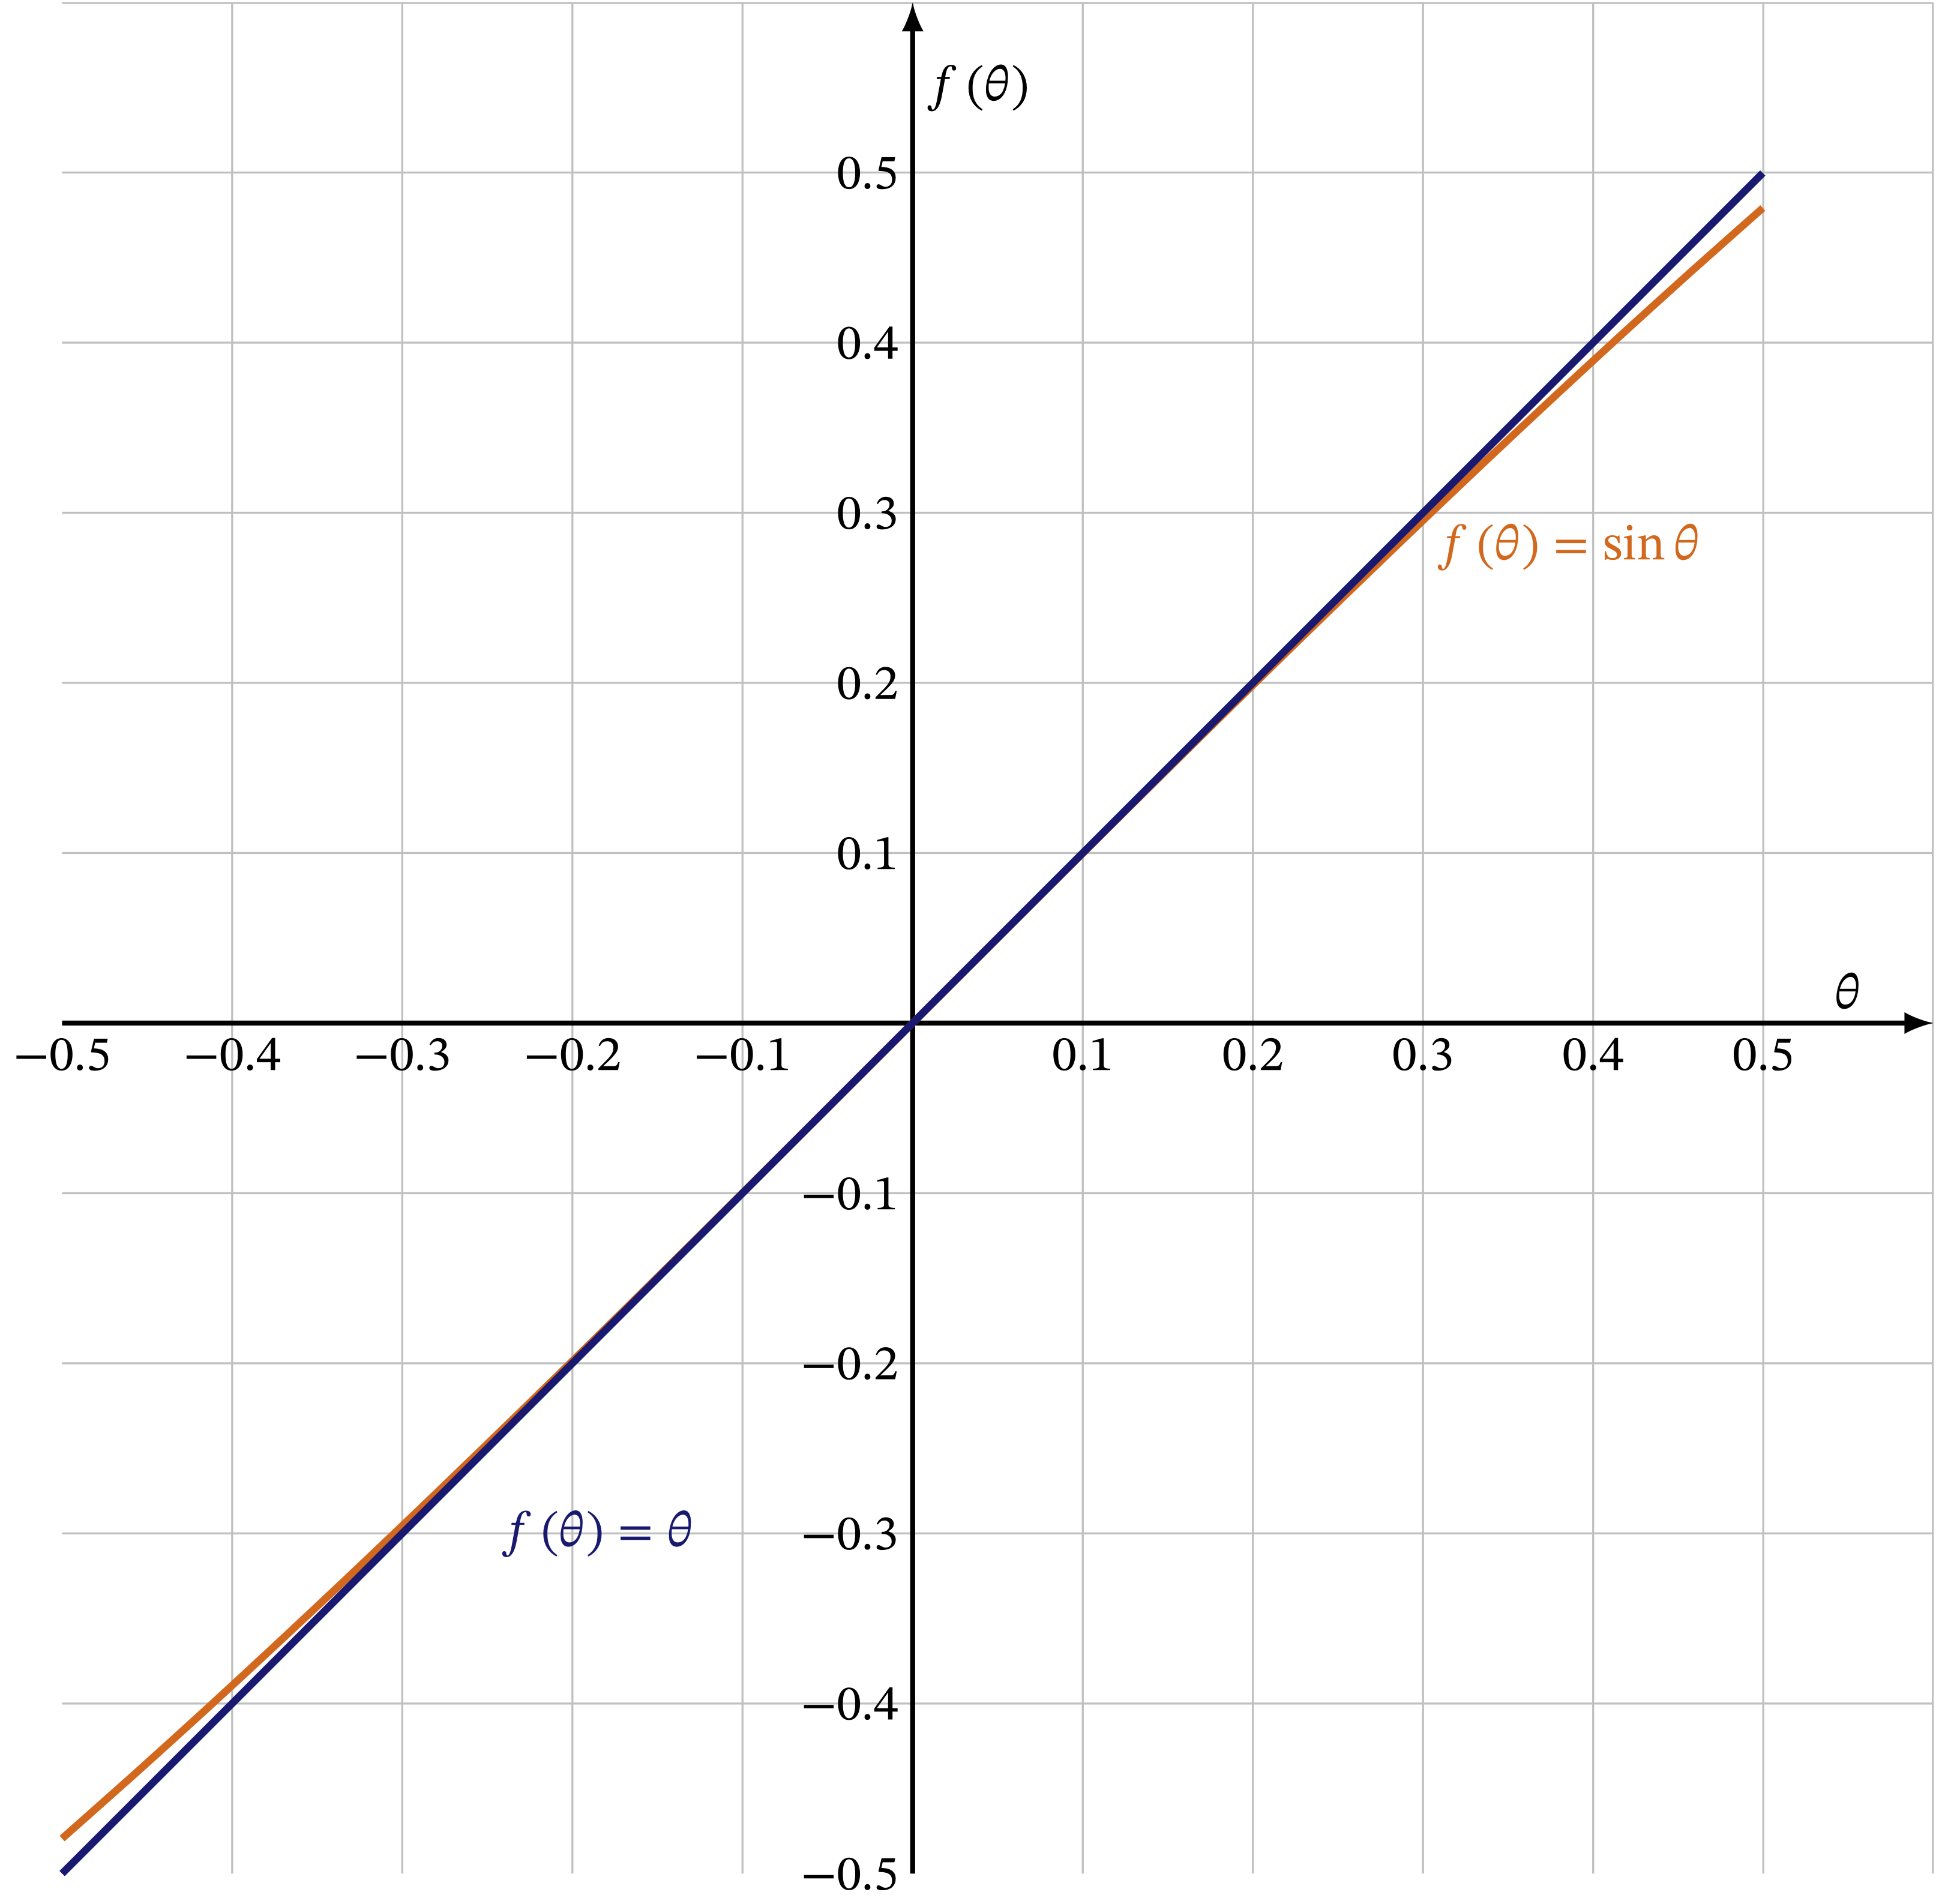
\includegraphics[width=0.9\textwidth,height=\textheight]{images/xsinx.png}
\caption{Graphs of \(f(\theta)= \sin\theta\) and \(f(\theta) = \theta\)
for \(\lvert\theta\rvert\approx 0\).}\label{fig:xsinx}
}
\end{figure}

Let us now illustrate the reasonableness of \cref{eq:sinesmalltheta} by
evaluation. Set \(\theta\) to \(0.005\) radians, which is a small value
close to zero. Then \(\sin\theta = \sin(0.005) = 0.004999979167\), which
demonstrates the validity of \cref{eq:sinesmalltheta}. However, if one
were to interpret the number 0.005 as degrees rather than radians, we
then have \(\sin(0.005°) = 0.00008726646249\) which is almost \(57\)
times smaller than the number 0.005.

The moral of this example is that when we evaluate trigonometric
functions in degrees in the context of their power series, we must apply
a correction factor of \(\frac{\pi}{180}\) to implicitly convert the
function argument on the LHS from degrees to radians. Otherwise, keeping
the degree argument, we have to apply a factor of \(\frac{180}{\pi}\) to
\emph{each term} on the RHS. This is a layer of bookkeeping we may
easily avoid by using radians on both sides of the equation.

\hypertarget{fourier-series}{%
\subsection{Fourier series}\label{fourier-series}}

Periodic waveforms repeat themselves indefinitely. The sinusoids---which
are trigonometric functions like \(\sin\) and \(\cos\)---are one such
example. Such waveforms arise frequently in signal analysis and
synthesis in electrical engineering. In that context, the independent
variable is \emph{time}.

A \emph{periodic function}
\href{https://eng.libretexts.org/Bookshelves/Electrical_Engineering/Signal_Processing_and_Modeling/Signals_and_Systems_(Baraniuk_et_al.)/06\%3A_Continuous_Time_Fourier_Series_(CTFS)/6.06\%3A_Convergence_of_Fourier_Series}{with
certain properties} may be represented by an infinite sum of sinusoids.
This was the great insight of
\href{https://en.wikipedia.org/wiki/Joseph_Fourier}{Jean-Baptiste Joseph
Fourier} from whom Fourier series derive their name.

For example, let the original signal be a square waveform denoted by the
function \(s(t)\) in \cref{fig:squarefourier}.\footnote{Strictly
  speaking, there are \emph{point discontinuities} in \(s(t)\), at
  \(t=\pi\) and \(t = 2\pi\), where the function changes value. The
  graph of the waveform is shown as a vertical line at these points
  because that is what an oscilloscope trace of the waveform will show.
  This is convenient but inaccurate because a \emph{function} cannot be
  multi-valued at one point. Nevertheless, the theory behind Fourier
  series is still applicable to the square wave. The Fourier series will
  converge at these points to zero---the average value at these
  discontinuities---which is what the partial sums show.} Imagine that
the single cycle of the square wave---shown below--- is repeated
periodically forever.

\begin{figure}
\hypertarget{fig:squarefourier}{%
\centering
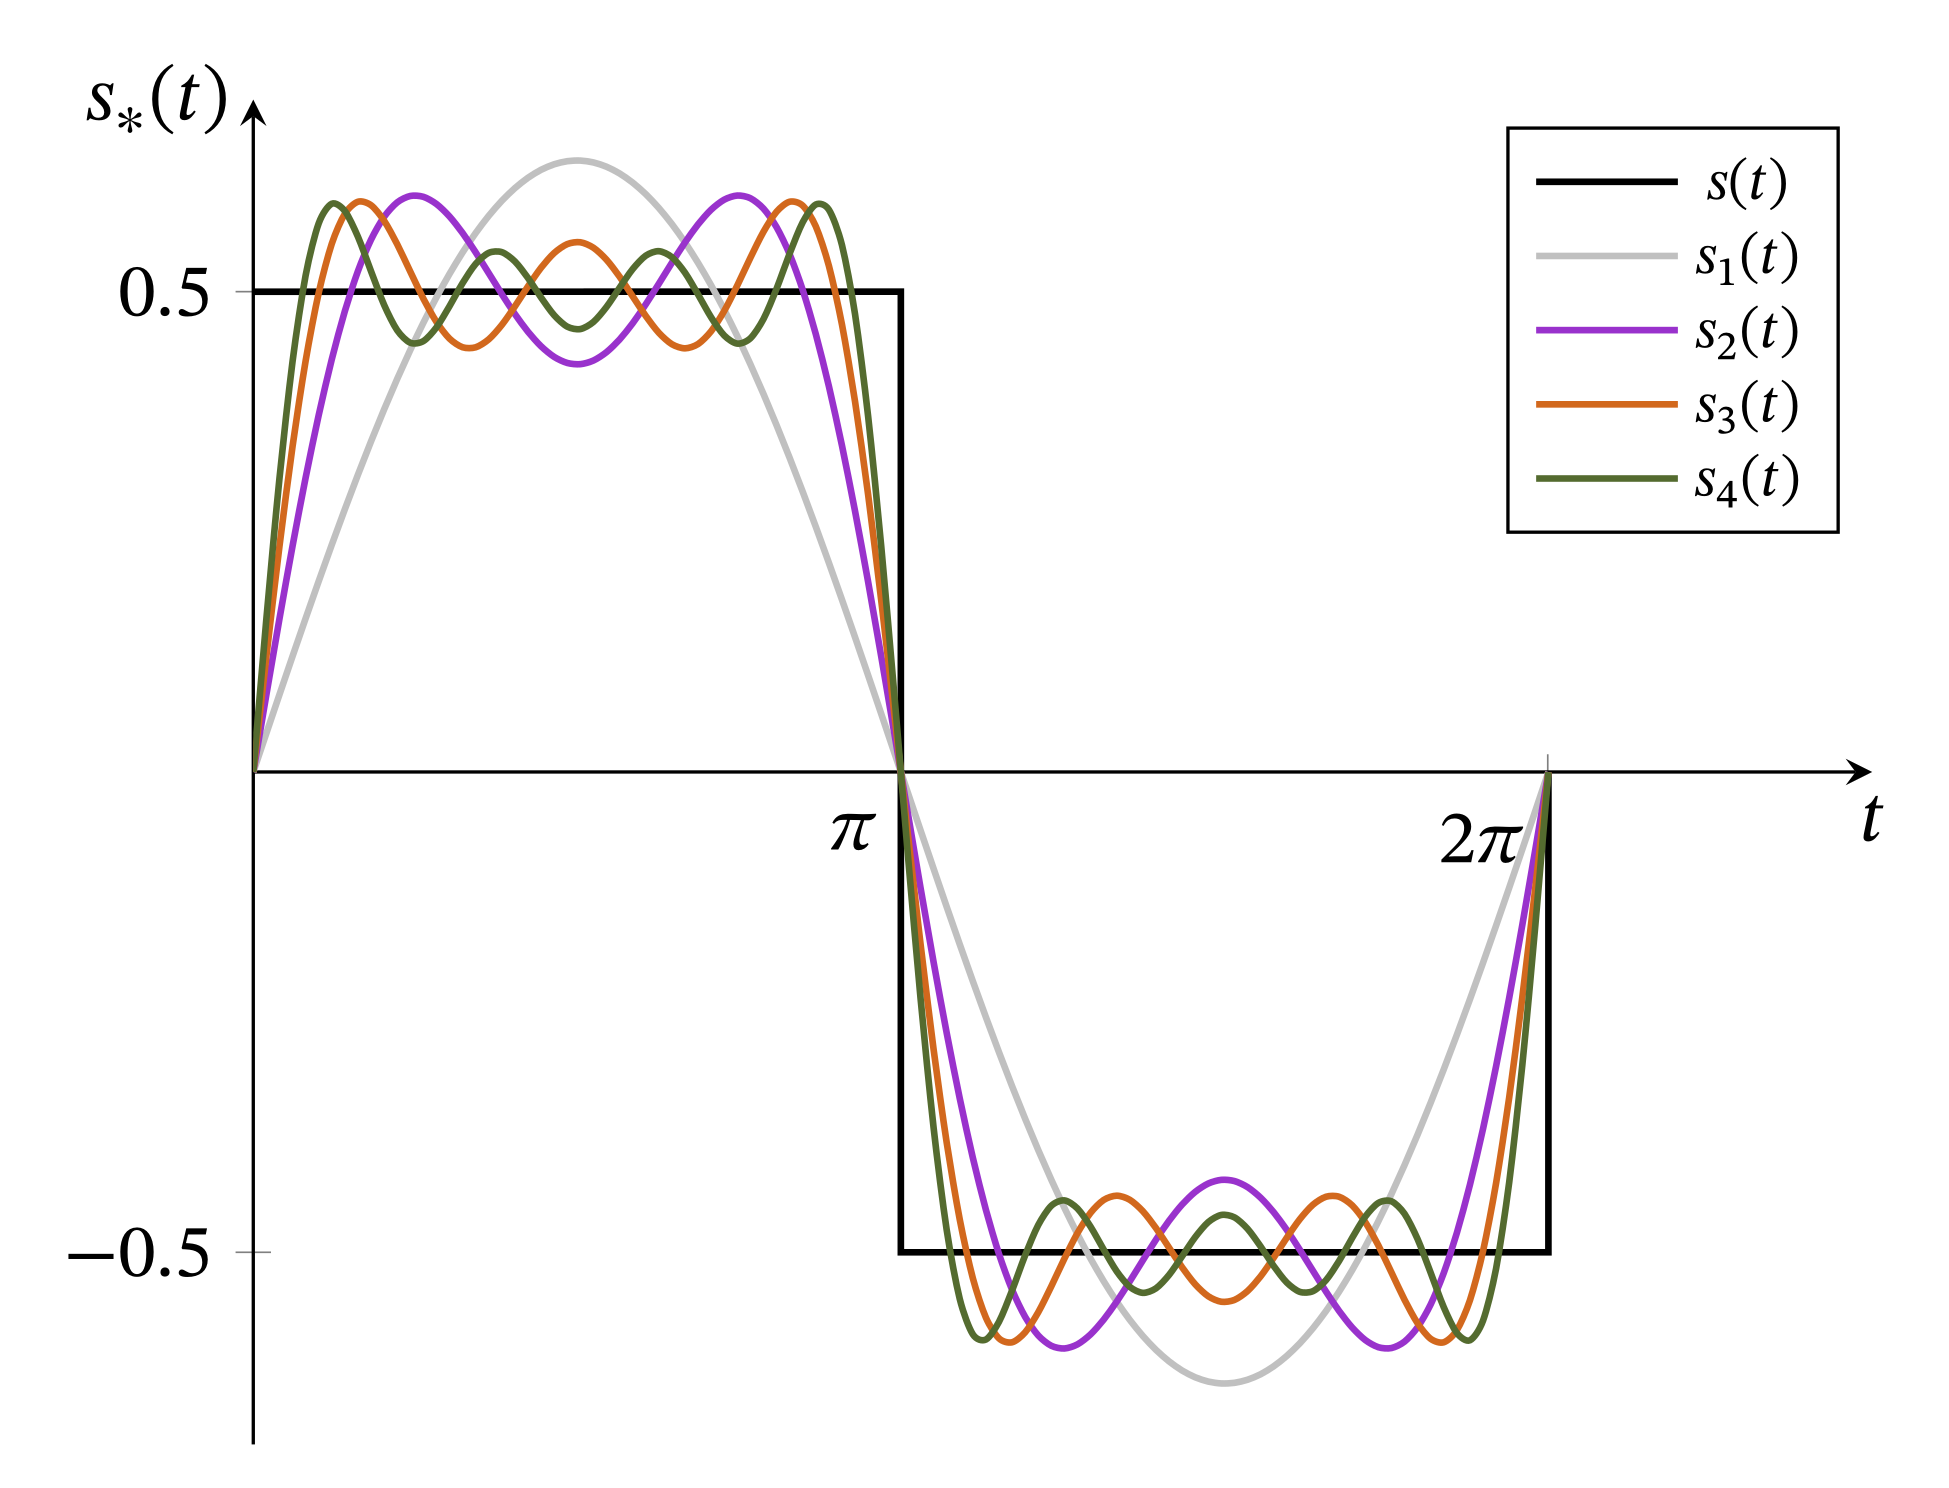
\includegraphics[width=0.85\textwidth,height=\textheight]{images/squarefourier.png}
\caption{A square waveform \(s(t)\) and the sequential sums of its first
four terms.}\label{fig:squarefourier}
}
\end{figure}

The \href{https://mathworld.wolfram.com/FourierSeries.html}{Fourier
series} for such a square waveform is an infinite sum of sinusoids that
collectively represent the waveform. This might seem like a tall order
but it is nevertheless true. The Fourier series representation of the
square wave \(s(t)\) is given by:
\begin{equation}\protect\hypertarget{eq:squarefourier}{}{
s(t) = \frac{2}{\pi}\left[\sin(t) + \frac{\sin(3t)}{3} + \frac{\sin(5t)}{5} +  \frac{\sin(7t)} {7} + \cdots\right]
}\label{eq:squarefourier}\end{equation} where again, the dots mean that
the pattern repeats forever. Note that this is no approximation, but an
equality.

The successive \emph{partial sums} of the RHS of \cref{eq:squarefourier}
are termed \(s_1(t)\), \(s_2(t)\), etc., with \(s_1(t)\) denoting the
first term, \(s_2(t)\), the sum of the first and second term etc. It is
evident from \cref{fig:squarefourier} that the more terms we add, the
better the match between the original signal and its approximation,
denoted generically by \(s_*(t)\) in the graph.\footnote{This
  property---where the larger the number of terms in the partial sum,
  the better the approximation to the original function---is one reason
  why Fourier series are widely applied.}

On the surface, \cref{eq:squarefourier} seems a remarkable claim. How
could a square wave with right angle corners be the result of sums of
sine waves which have no corners? The answer lies in the fact that the
series goes on forever and ``infinity confers the equality''.

Where do radians feature here? As with the power series for the sine
function, it is on the RHS where the variable \(t\) should be expressed
in radians. Note that while \(t\) may have units of time, the fact that
radians are unitless does not intrude into the equation as an extraneous
factor.

We will close with one more example where radians make mathematical life
much easier.

\hypertarget{eulers-formula-and-identity}{%
\subsection{Euler's formula and
identity}\label{eulers-formula-and-identity}}

The prodigiously productive Swiss mathematician,
\href{https://www.britannica.com/biography/Leonhard-Euler}{Leonhard
Euler}, gave us many equations, one of which is known as \emph{Euler's
formula}, shown below: \begin{equation}\protect\hypertarget{eq:euler}{}{
e^{i\theta} = \cos\theta + i\sin\theta
}\label{eq:euler}\end{equation} The letter \(i\) is called the
\href{https://en.wikipedia.org/wiki/Imaginary_unit}{imaginary unit} and
its definition as \(i^{2} = -1\), takes us into the
\href{https://en.wikipedia.org/wiki/Complex_number}{field of complex
numbers}\footnote{\href{https://en.wikipedia.org/wiki/Fundamental_theorem_of_algebra}{The
  Fundamental Theorem of Algebra} states that all non-constant
  polynomials with complex coefficients contain at least one complex
  root, to express which \(i\) is necessary.}.

When we substitute \(\theta=\pi\) into \cref{eq:euler}, and transpose
terms, we get what is called \emph{Euler's identity}:
\begin{equation}\protect\hypertarget{eq:euleridentity}{}{
\begin{aligned}
e^{i\pi} &= \cos\pi + i\sin\pi\\
e^{i\pi} + 1 &= 0\\
\end{aligned}
}\label{eq:euleridentity}\end{equation}

\cref{eq:euleridentity} has been described as the most poetic
mathematical equation because it
\href{https://www.livescience.com/51399-eulers-identity.html}{unites in
one equation the five most fundamental quantities in all of
mathematics}: \(e, i, \pi, 1\) and \(0\). And it could not have come
about without radians. With that
\href{https://www.thefreedictionary.com/epiphany}{epiphany} on beauty,
we shall conclude our tale of two measures.

\hypertarget{acknowledgements}{%
\subsection{Acknowledgements}\label{acknowledgements}}

All illustrations in this blog were generated using the
\href{https://github.com/pgf-tikz/pgf}{TikZ-PGF} and
\href{https://pgfplots.sourceforge.net/}{PGFPlots} packages with
\href{https://www.latex-project.org/}{LaTeX} and
\href{https://pandoc.org/}{Pandoc}. To the authors of these packages,
and to others who posted numerous examples of their usage on the Web, my
humble gratitude. For \cref{fig:squarefourier}, I have drawn upon and
modified the \href{https://tex.stackexchange.com/a/429505/1636}{example
of caverac} at the \href{https://tex.stackexchange.com/}{TeX
StackExchange} forum.

\hypertarget{feedback}{%
\subsection{Feedback}\label{feedback}}

Please \href{mailto:feedback.swanlotus@gmail.com}{email me} your
comments and corrections.

\noindent A PDF version of this article is
\href{./radians.pdf}{available for download here}:

\begin{small}

\begin{sffamily}

\url{https://swanlotus.netlify.app/blogs/radians.pdf}

\end{sffamily}

\end{small}



\end{document}
